\section{Estimating parameters Activation energies for reaction 2  and 3  }

The results displayed in this section are for the uncertainty involved in the calculation of flamespeed depending on two parameters i.e the activation energy for the fall off reaction and activation energy for reaction 2 in the ozone mechanism. The percentage of ozone is taken  20,28,40,46,53,75 and 100  percent acccording to the experimental data available to us from Streng\cite{Streng}.The results are dispalyed in three section. In first section, for constant surrogate size, the number of samples are changes. In the second part of the results, convergence study is done for all samples with surrogate size 100*100. In third section, we ensure that samples of the parameters which we are drawing are fitting the flamespeed values of the experiment. Also for varying size the map point of the resulting pdf does not change greatly. The surrogates for individual concentrations are constructed using linear interpolation function. The initial guess for the map point is calculated using nelder mead optimization technique. After supplying initial guess over large domain it is found that the map point is the same no matter where we start our guess. 
\bigskip

\subsection{Different surrogate sizes }

\noindent Here the surrogate size is defined as $sample size*2$ matrix. The flamespeed is calculated for given samples in the domain ( -10 to 40) for $E_2$ and in the domain ( -10 to 40) for $E_3$. Other values are calculated as linear interpolation of these 1000 points. In this analysis, raw chain size of $1e5$, $5e5$ , $1e6$, $5e6$ and $1e7$ is taken. 

\subsubsection{Sample size (Surrogate size) 10*10 }
In this section we calculated flamespeed values for 100 (10*10) different points in the domain and the remaining values are linear combination of these 100 points.  The results below are for sample size $1e5$, $5e5$ , $1e6$, $5e6$ and $1e7$. 

\begin{figure}[H]
\centering
\subfloat[MCMC raw chain of samples of $E_2$\label{subfig-1:dummy}]{%
     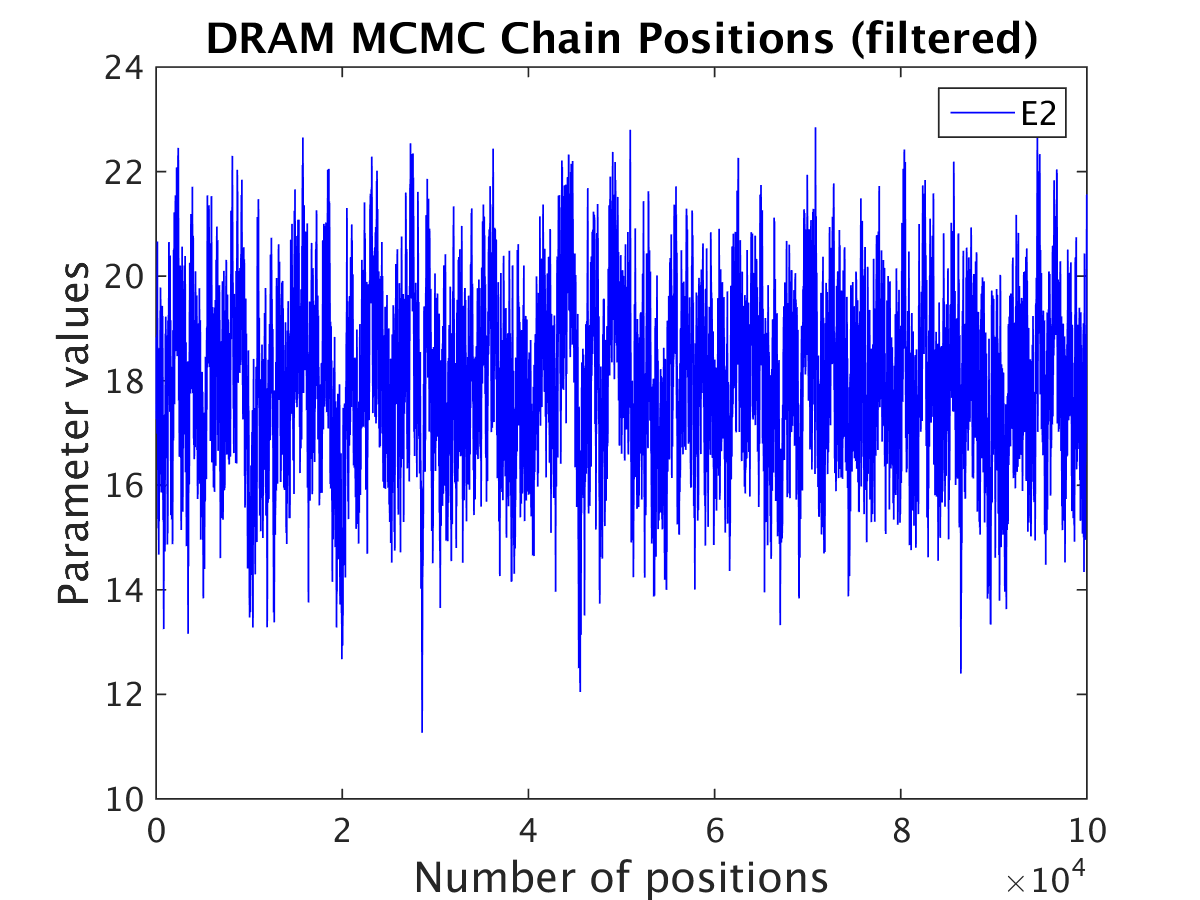
\includegraphics[scale=0.7]{multiple_data/10_kde/outputData_1e5/simple_ip_chain_pos_raw_1} 
    }
    \quad
    \subfloat[MCMC raw chain of samples of $E_2$\label{subfig-1:dummy}]{%
         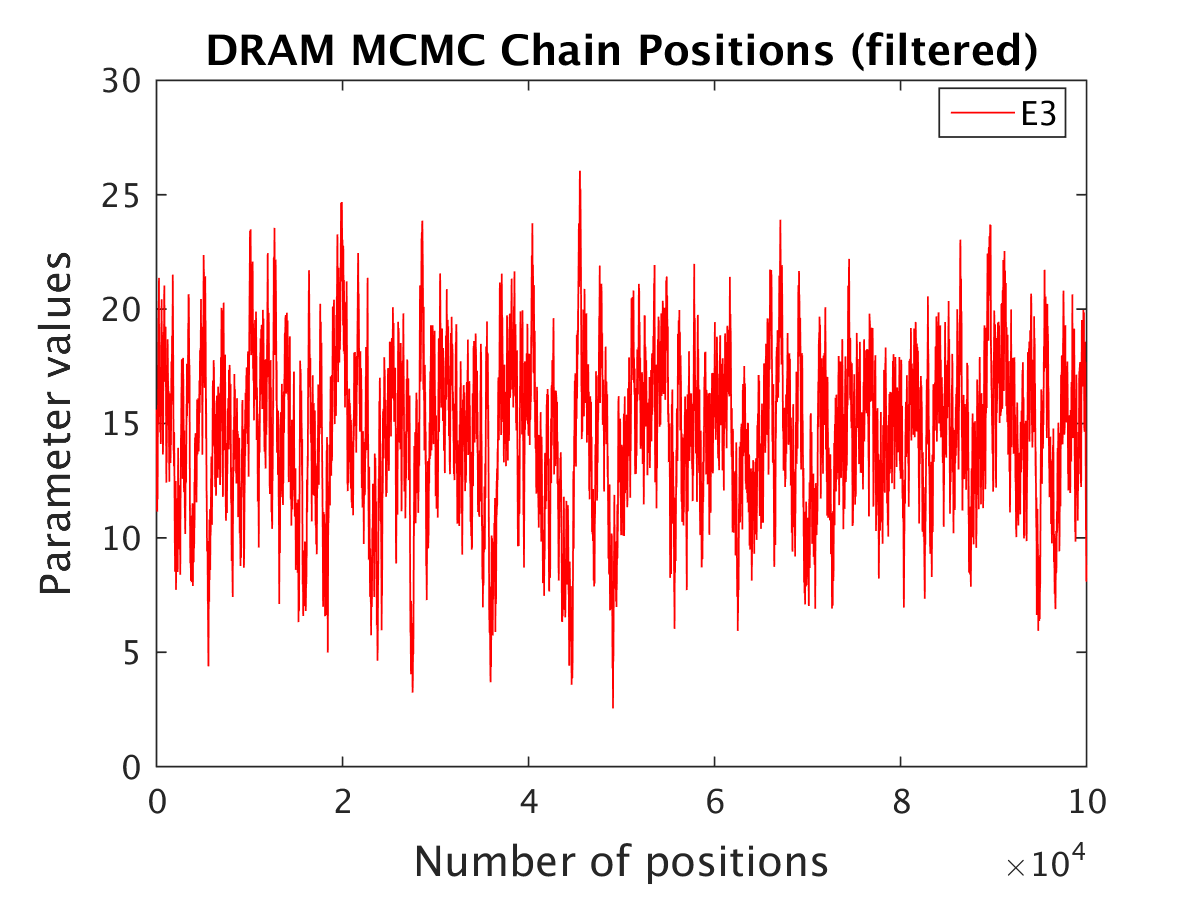
\includegraphics[scale=0.7]{multiple_data/10_kde/outputData_1e5/simple_ip_chain_pos_raw_2} 
        }
    \end{figure}
  \begin{figure}[H]
  \ContinuedFloat
  \centering
  \subfloat[Histogram for $E_2$ \label{subfig-1:dummy}]{%
       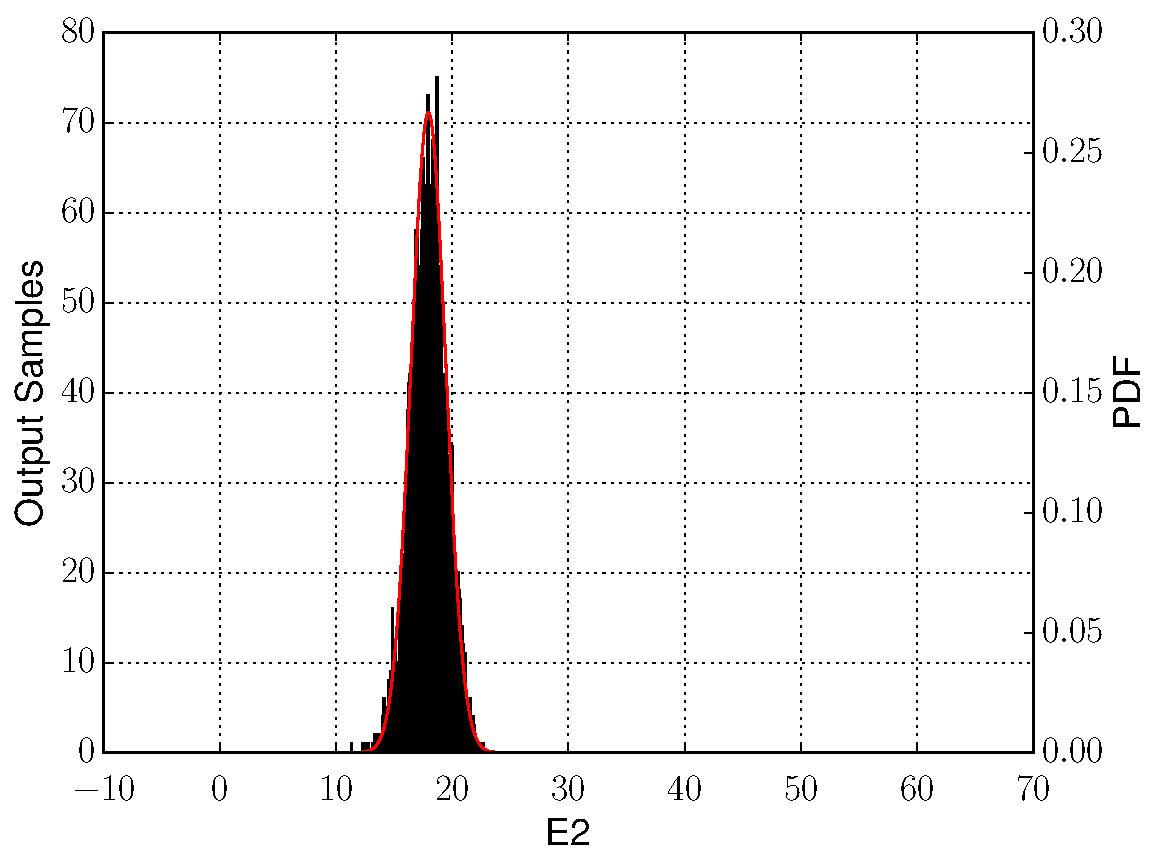
\includegraphics[scale=0.7]{multiple_data/10_kde/outputData_1e5/E2.pdf} 
      }
   \quad
    \subfloat[Histogram for $E_3$ \label{subfig-1:dummy}]{%
          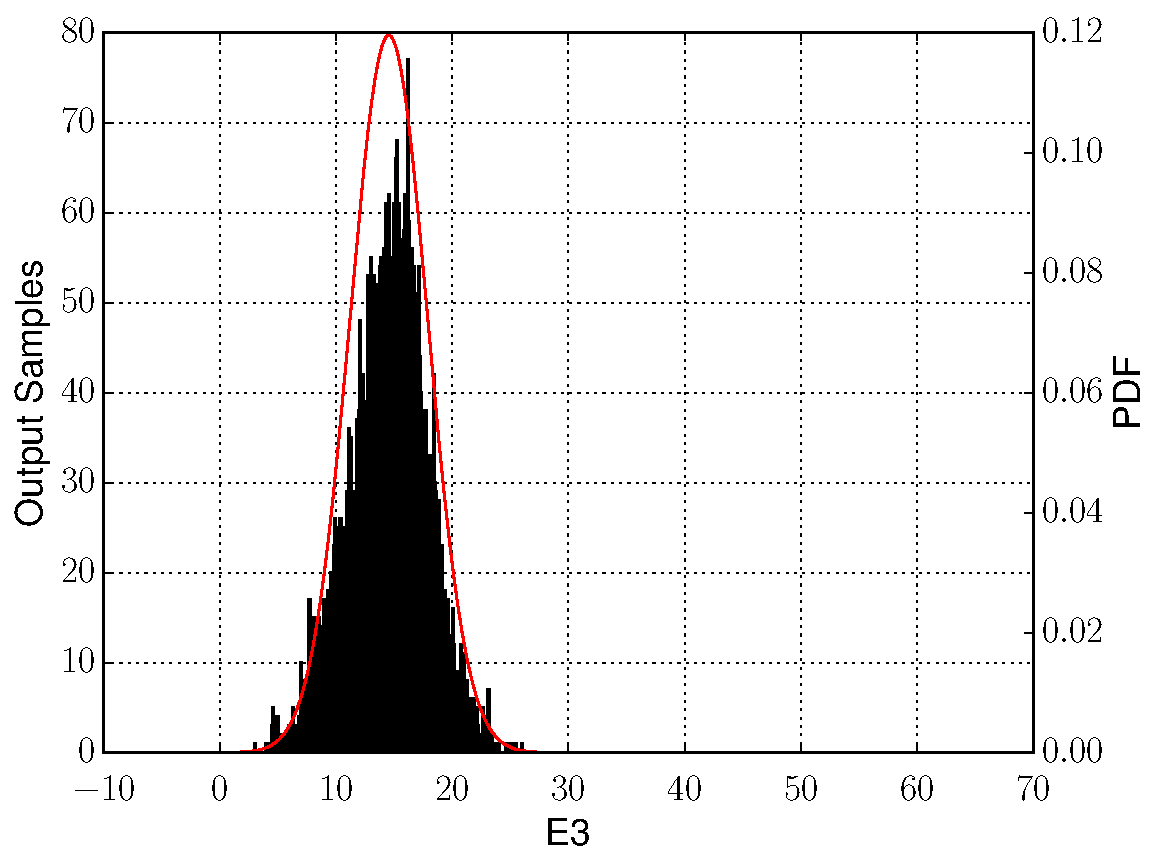
\includegraphics[scale=0.7]{multiple_data/10_kde/outputData_1e5/E3.pdf} 
         }
\end{figure}
\begin{figure}[H]
  
   \subfloat[Cummulative Density Funtion \label{subfig-1:dummy}]{
        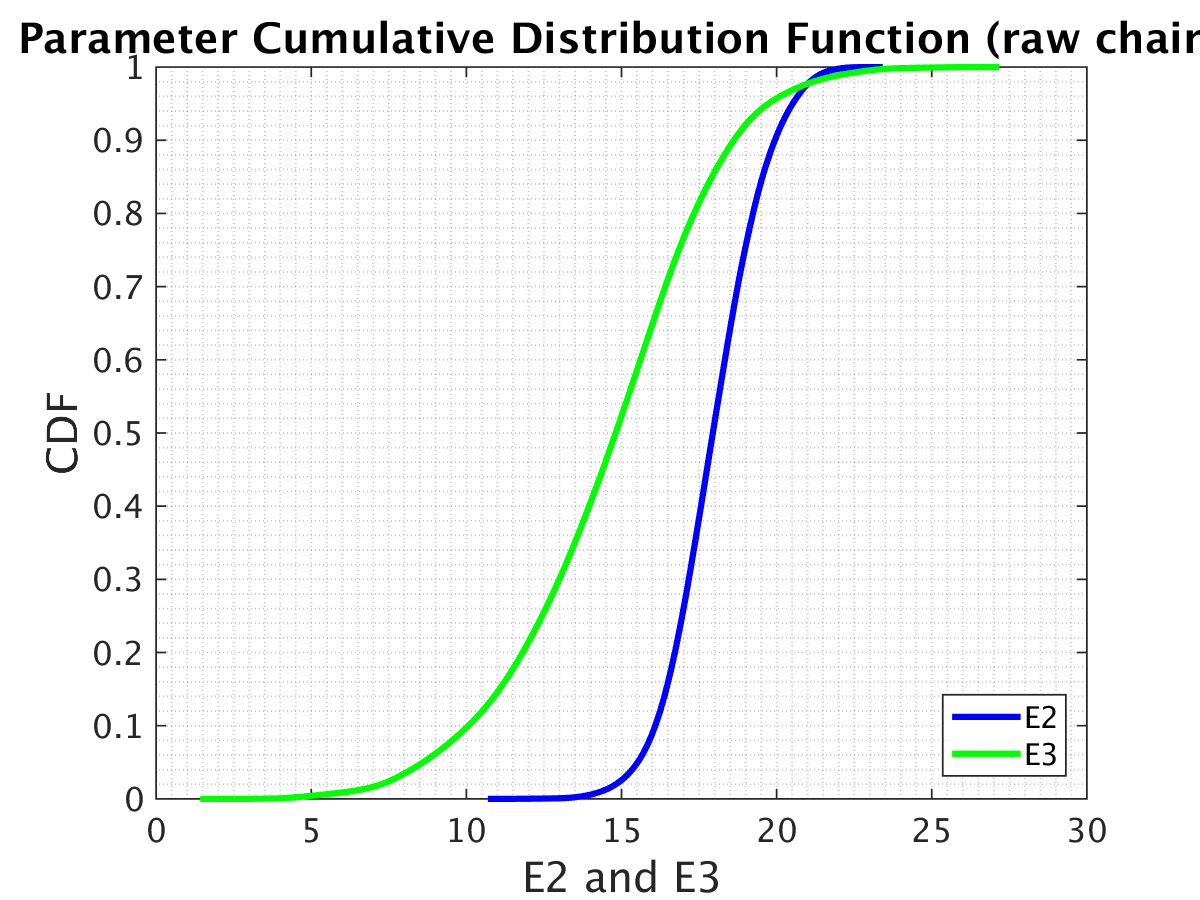
\includegraphics[scale=0.7]{multiple_data/10_kde/outputData_1e5/cdf} 
       }
     \quad
\subfloat[KDE \label{subfig-1:dummy}]{
        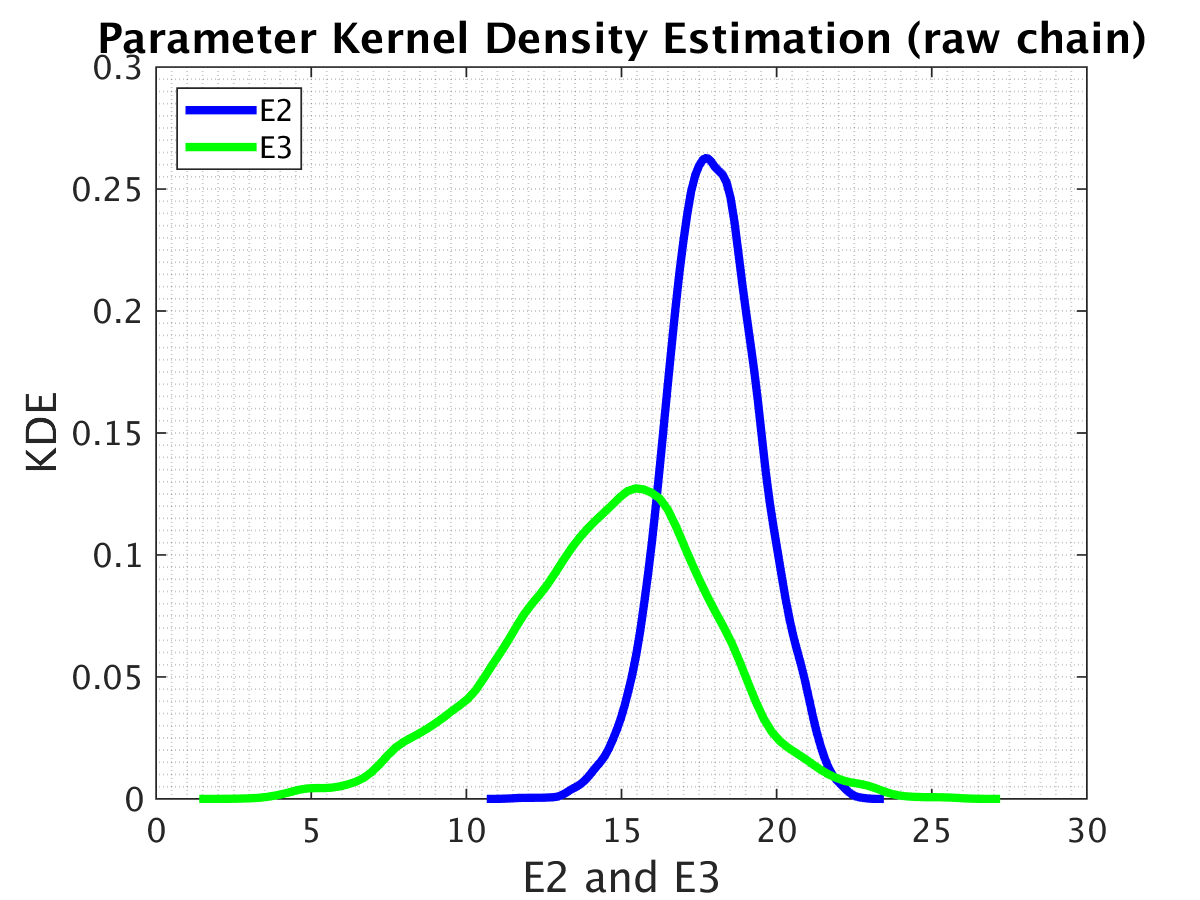
\includegraphics[scale=0.7]{multiple_data/10_kde/outputData_1e5/kde} 
            }  
  \caption{Results for sample size 1e5}
\end{figure}

\begin{figure}[H]
\centering
\subfloat[MCMC raw chain of samples of $E_2$\label{subfig-1:dummy}]{%
     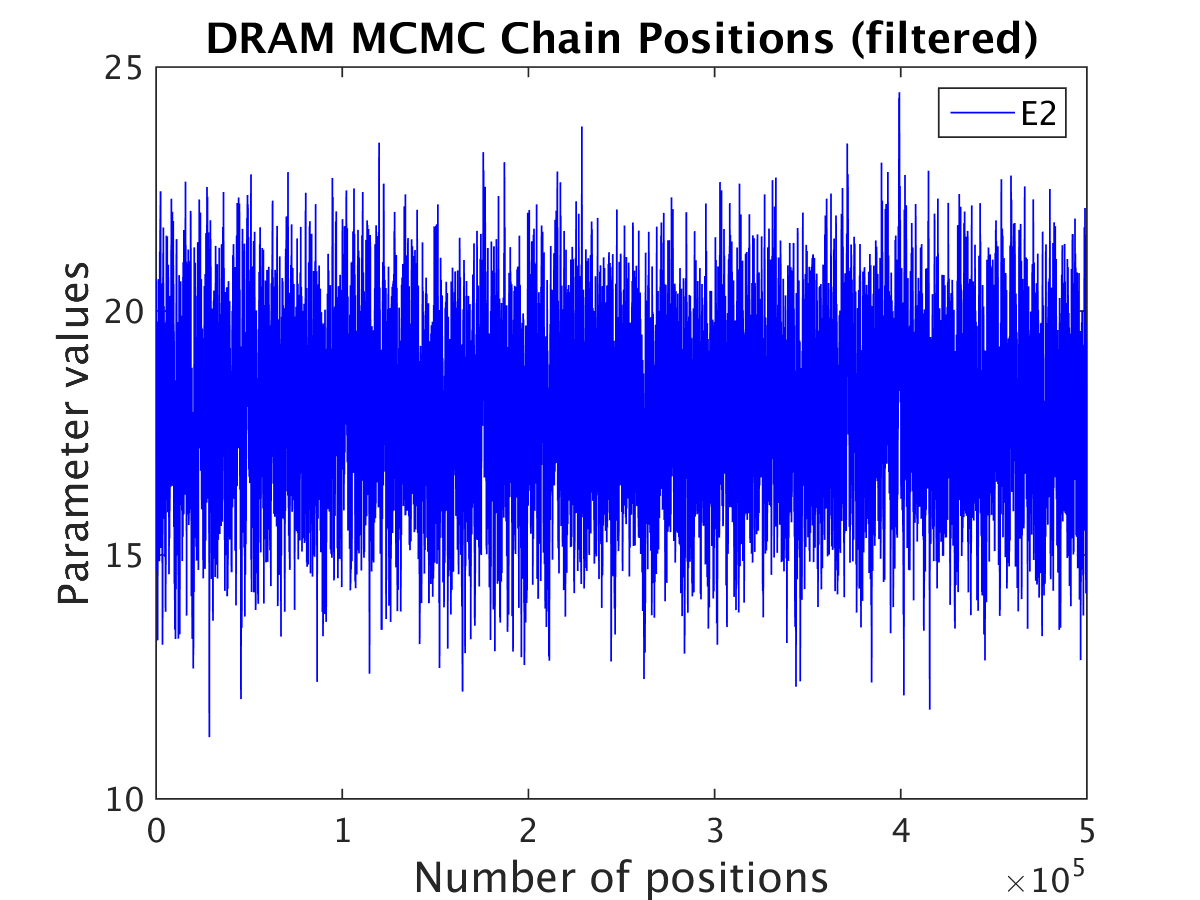
\includegraphics[scale=0.7]{multiple_data/10_kde/outputData_5e5/simple_ip_chain_pos_raw_1} 
    }
    \quad
    \subfloat[MCMC raw chain of samples of $E_2$\label{subfig-1:dummy}]{%
         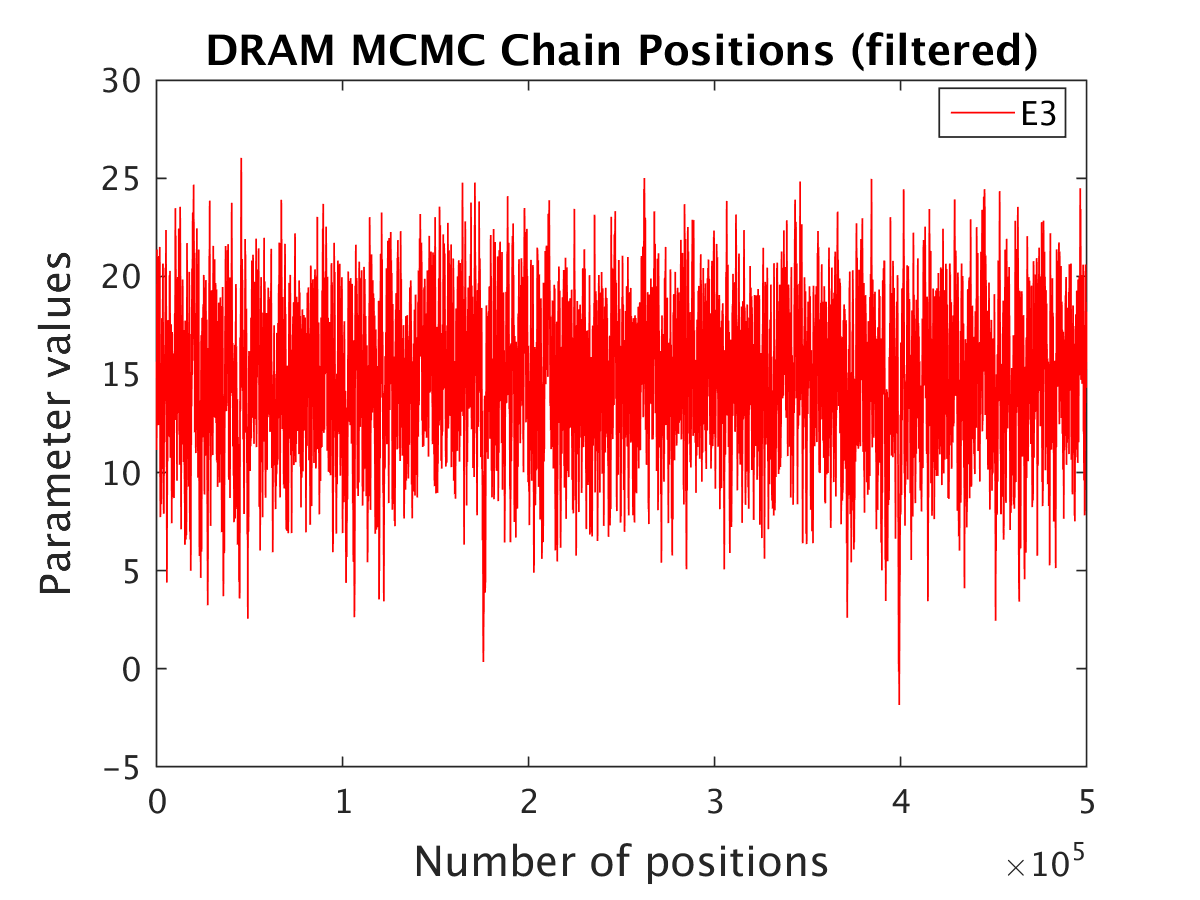
\includegraphics[scale=0.7]{multiple_data/10_kde/outputData_5e5/simple_ip_chain_pos_raw_2} 
        }
    \end{figure}
  \begin{figure}[H]
  \ContinuedFloat
  \centering
  \subfloat[Histogram for $E_2$ \label{subfig-1:dummy}]{%
       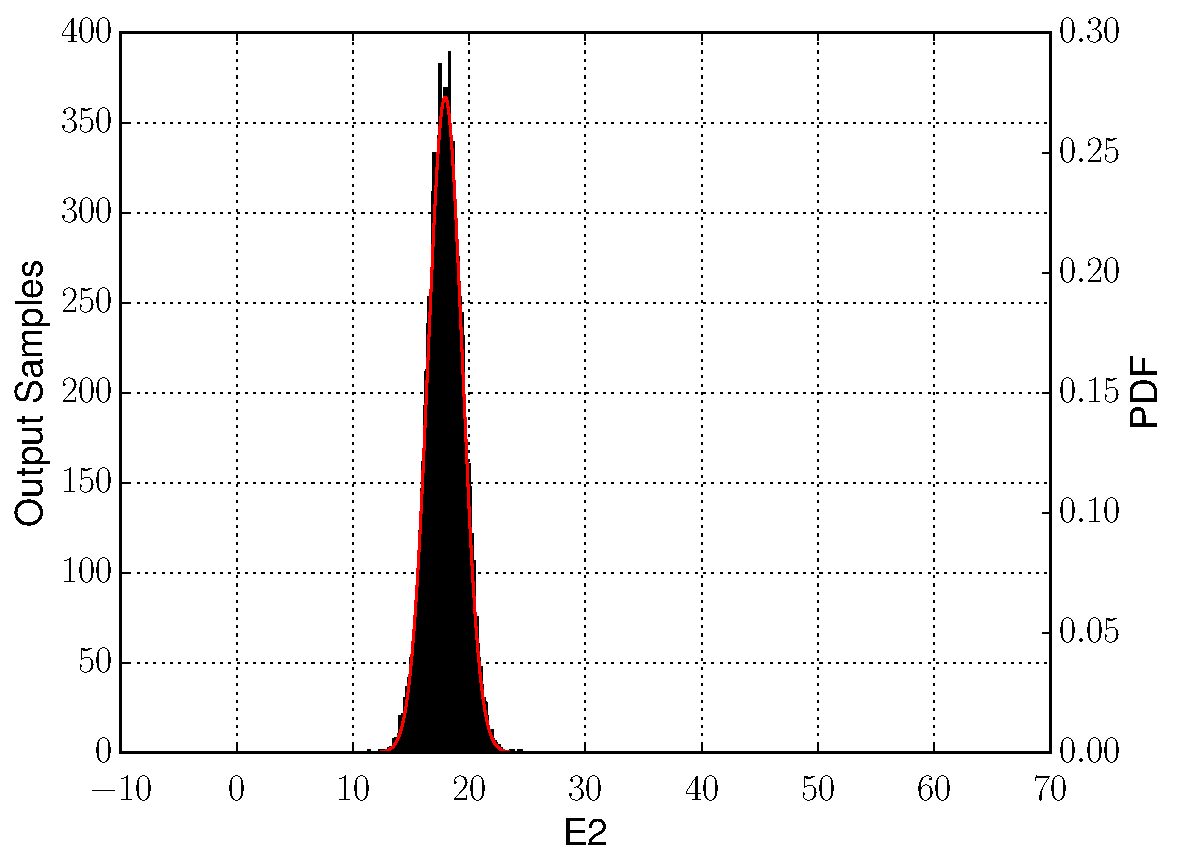
\includegraphics[scale=0.7]{multiple_data/10_kde/outputData_5e5/E2.pdf} 
      }
   \quad
    \subfloat[Histogram for $E_3$ \label{subfig-1:dummy}]{%
          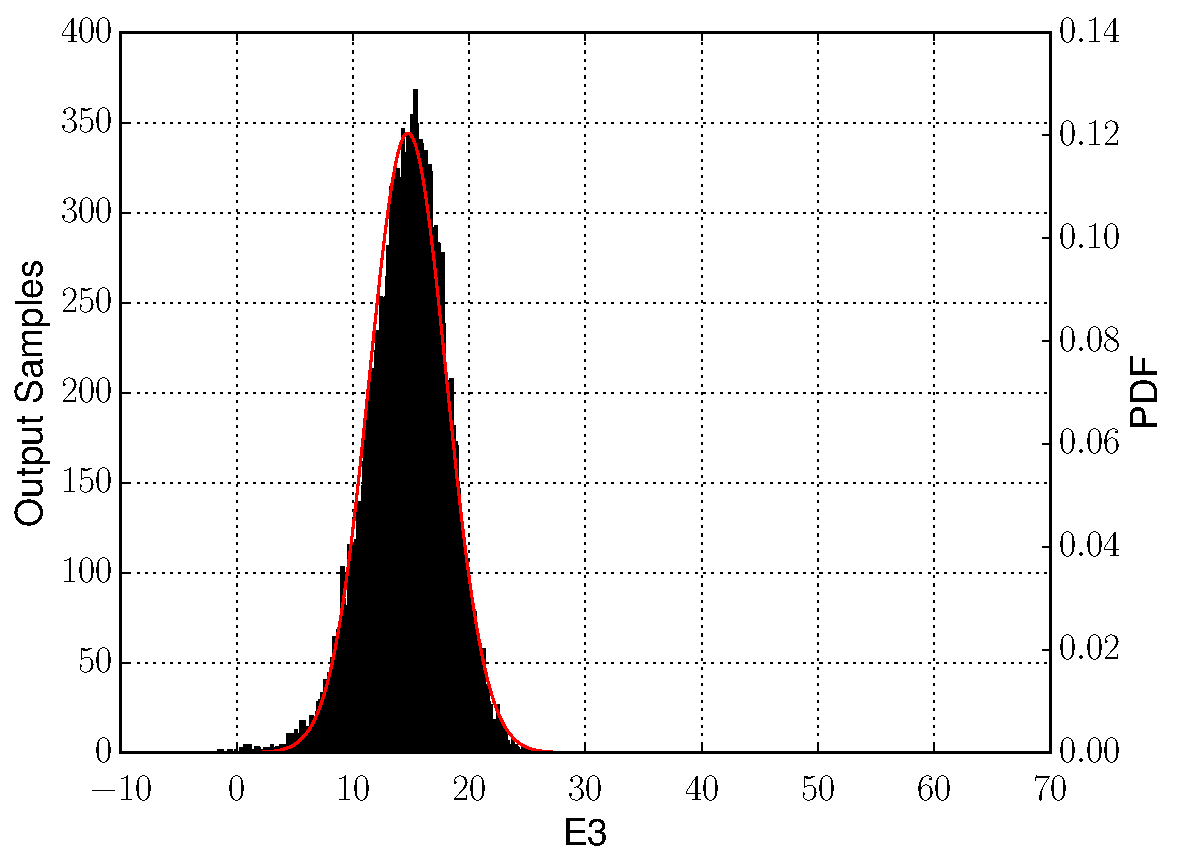
\includegraphics[scale=0.7]{multiple_data/10_kde/outputData_5e5/E3.pdf} 
         }
\end{figure}
\begin{figure}[H]
  
   \subfloat[Cummulative Density Funtion \label{subfig-1:dummy}]{
        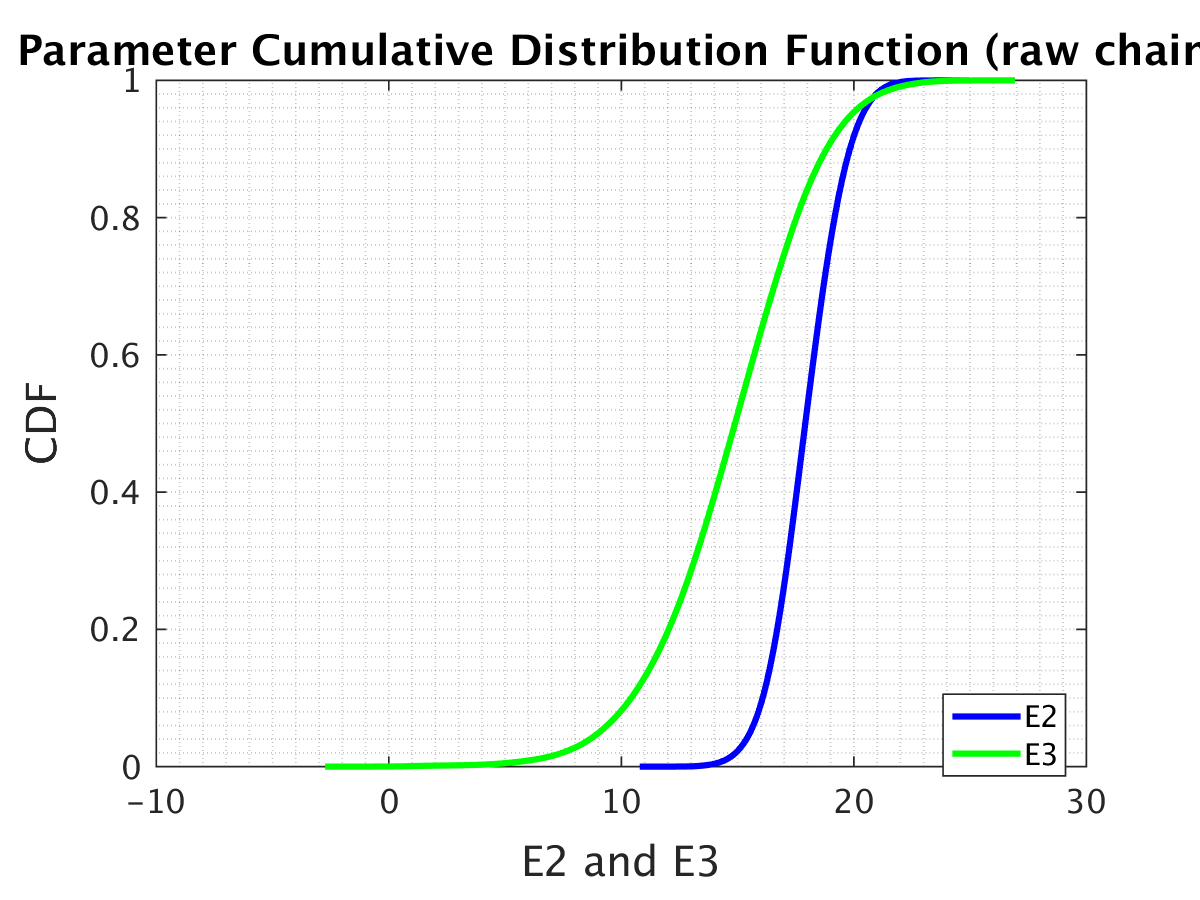
\includegraphics[scale=0.7]{multiple_data/10_kde/outputData_5e5/cdf} 
       }
     \quad
\subfloat[KDE \label{subfig-1:dummy}]{
        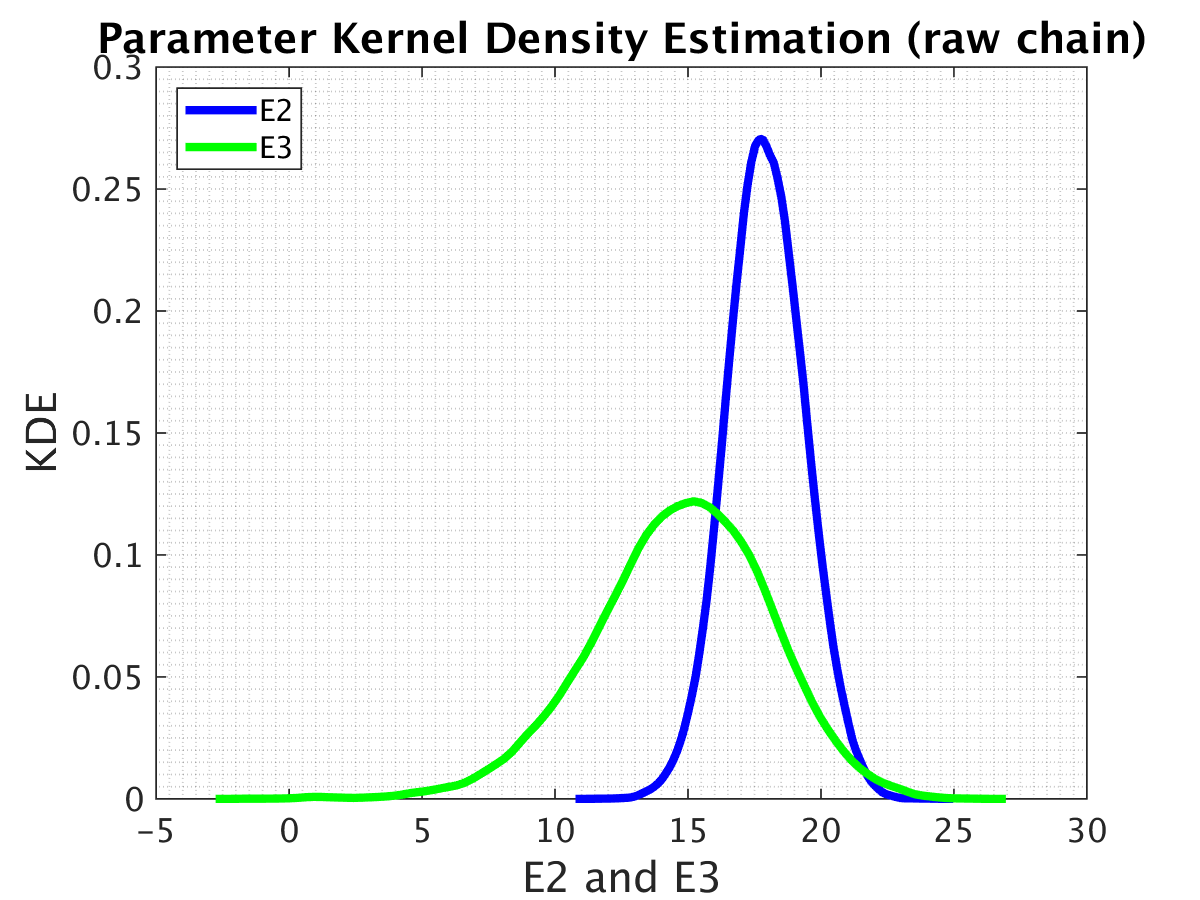
\includegraphics[scale=0.7]{multiple_data/10_kde/outputData_5e5/kde} 
            }  
  \caption{Results for sample size 5e5}
\end{figure}


\begin{figure}[H]
\centering
\subfloat[MCMC raw chain of samples of $E_2$\label{subfig-1:dummy}]{%
     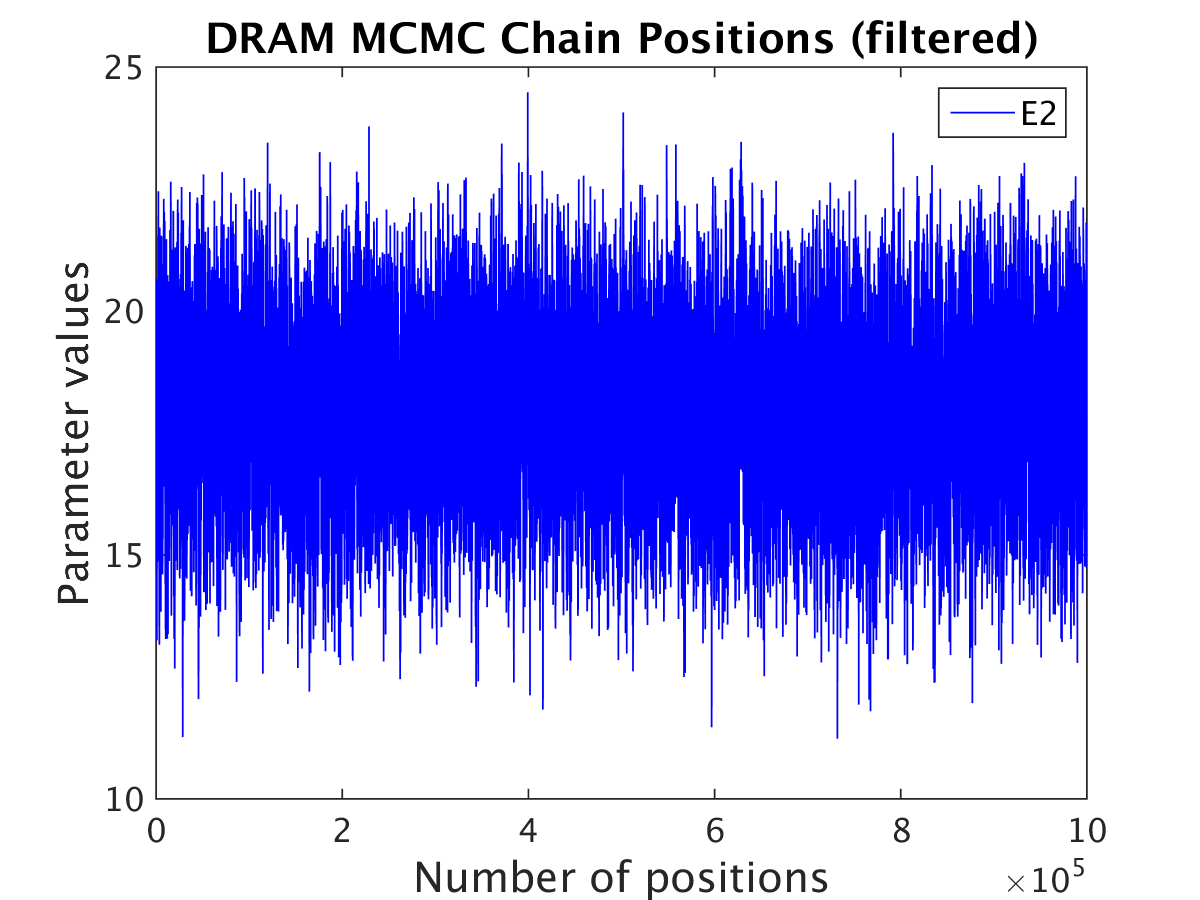
\includegraphics[scale=0.7]{multiple_data/10_kde/outputData_1e6/simple_ip_chain_pos_raw_1} 
    }
    \quad
    \subfloat[MCMC raw chain of samples of $E_2$\label{subfig-1:dummy}]{%
         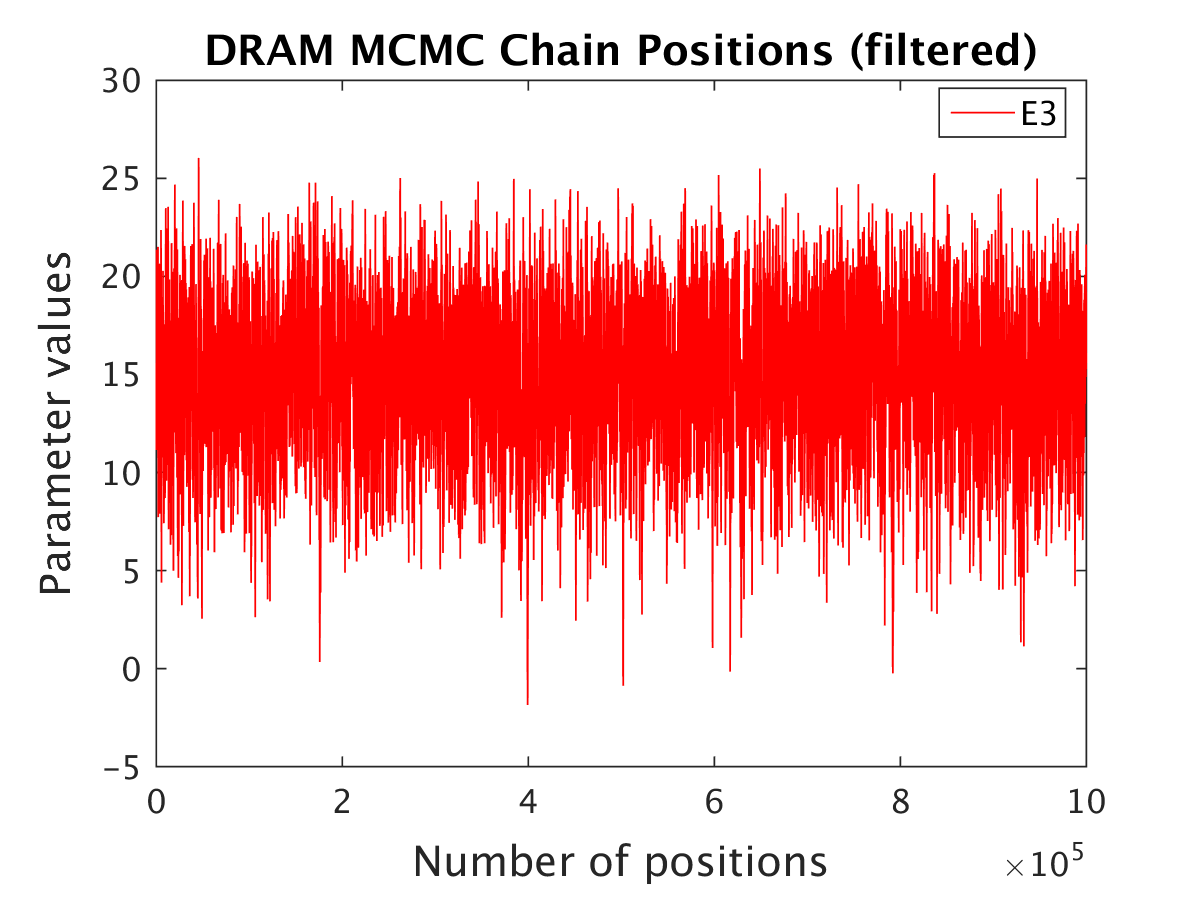
\includegraphics[scale=0.7]{multiple_data/10_kde/outputData_1e6/simple_ip_chain_pos_raw_2} 
        }
    \end{figure}
  \begin{figure}[H]
  \ContinuedFloat
  \centering
  \subfloat[Histogram for $E_2$ \label{subfig-1:dummy}]{%
       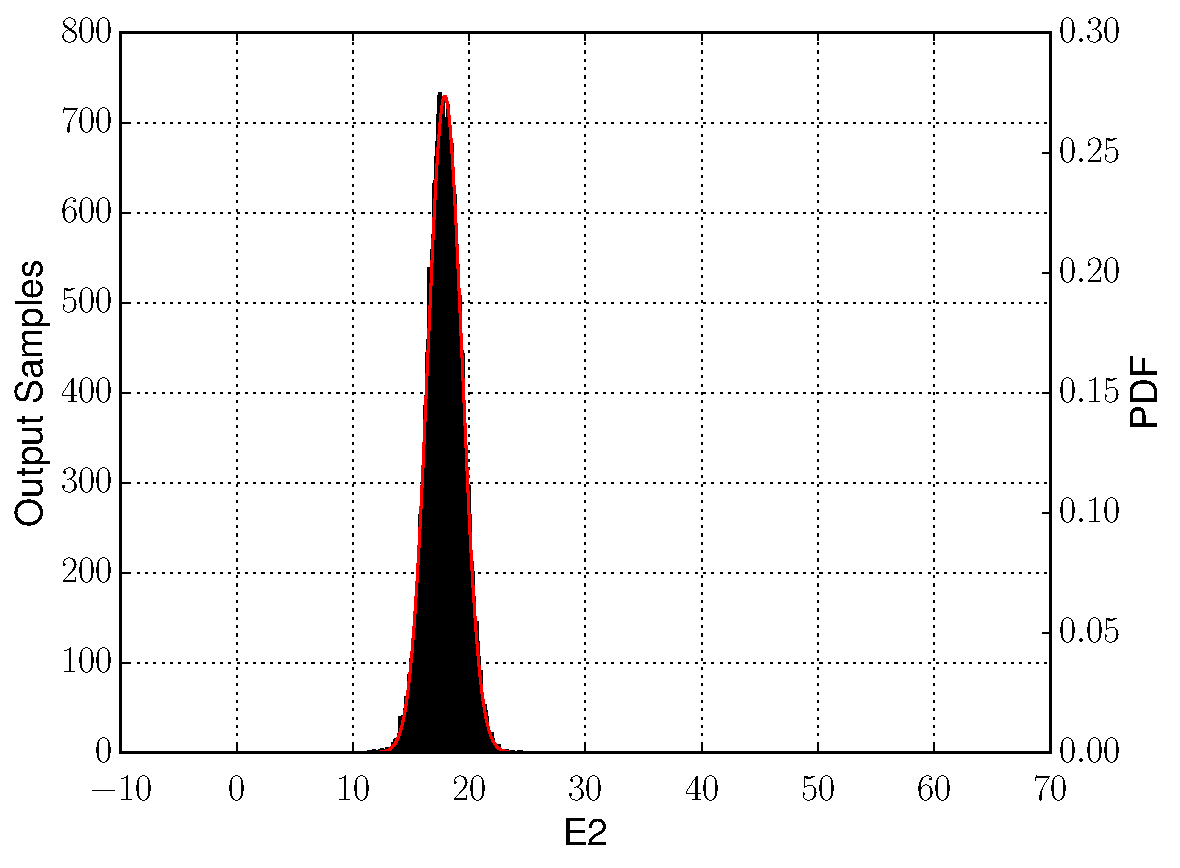
\includegraphics[scale=0.7]{multiple_data/10_kde/outputData_1e6/E2.pdf} 
      }
   \quad
    \subfloat[Histogram for $E_3$ \label{subfig-1:dummy}]{%
          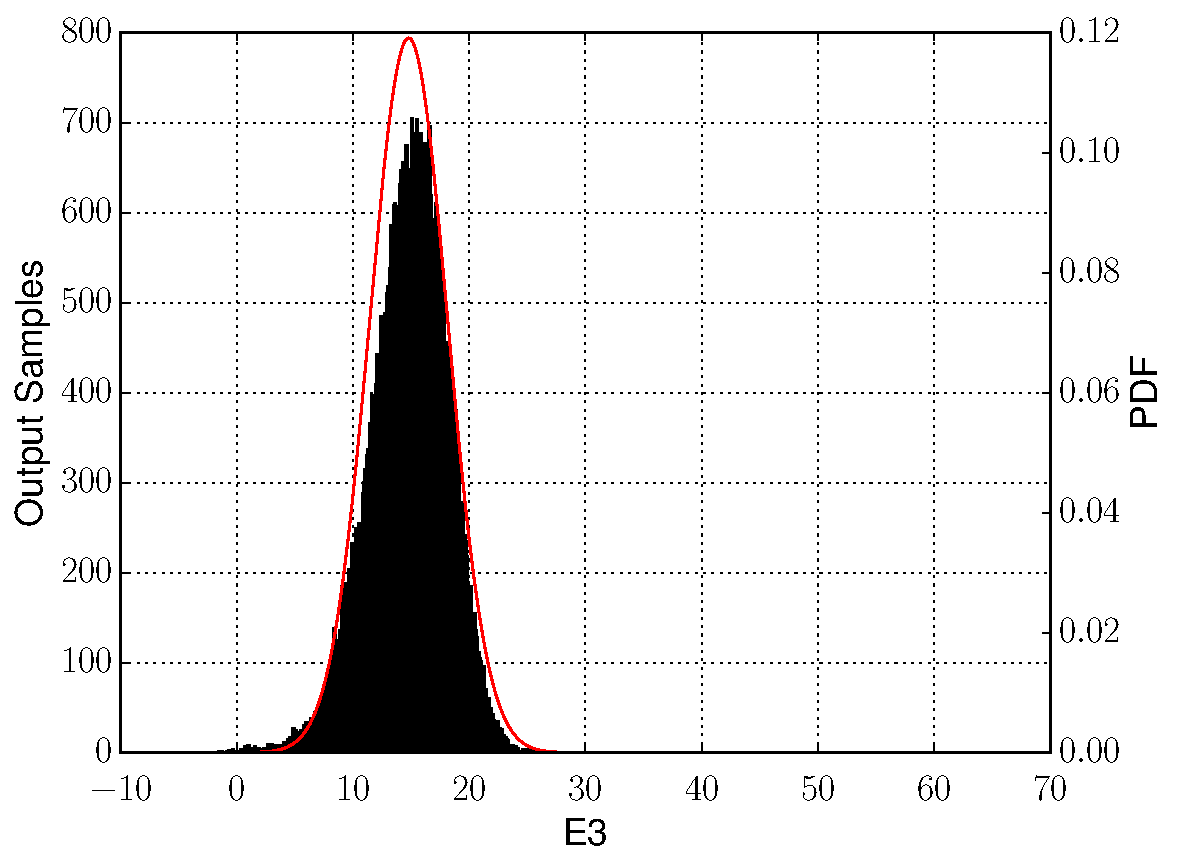
\includegraphics[scale=0.7]{multiple_data/10_kde/outputData_1e6/E3.pdf} 
         }
\end{figure}
\begin{figure}[H]
  
   \subfloat[Cummulative Density Funtion \label{subfig-1:dummy}]{
        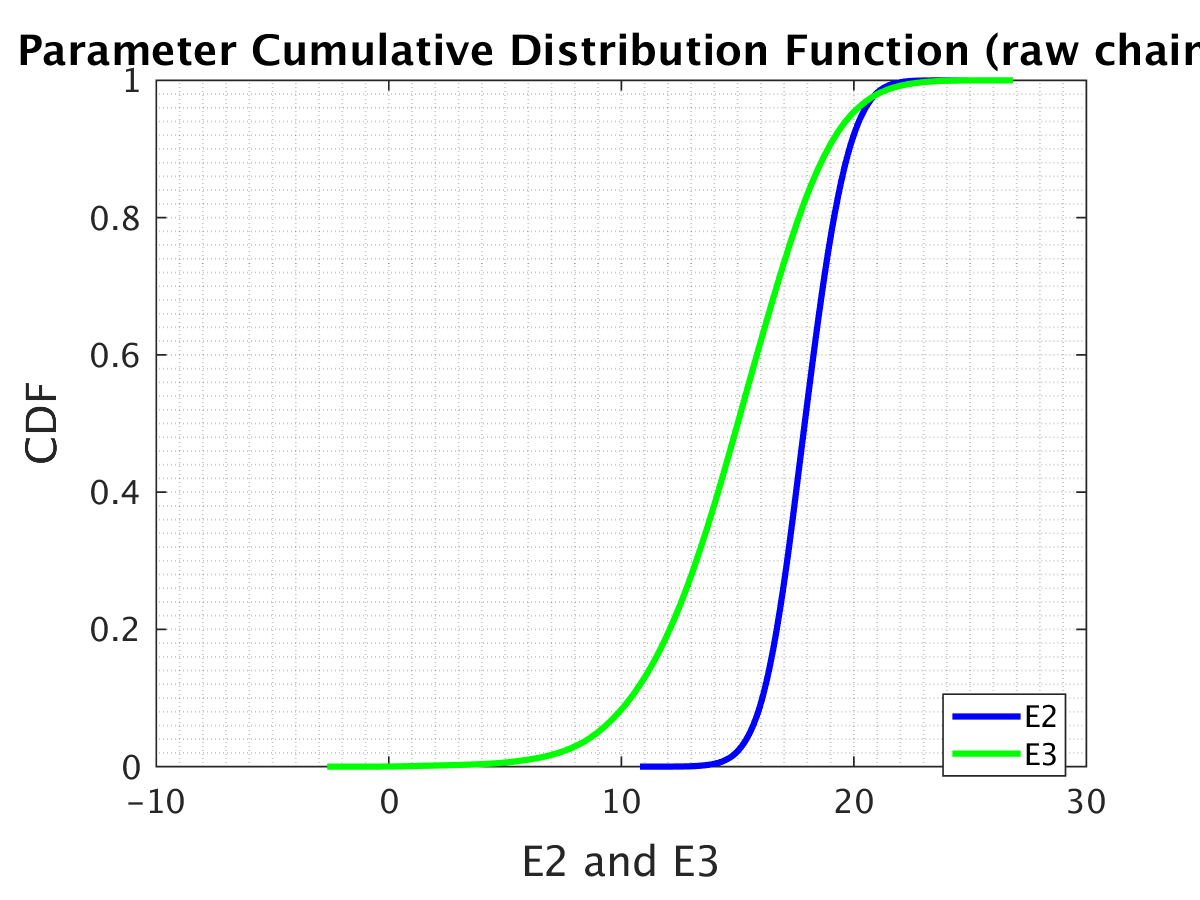
\includegraphics[scale=0.7]{multiple_data/10_kde/outputData_1e6/cdf} 
       }
     \quad
\subfloat[KDE \label{subfig-1:dummy}]{
        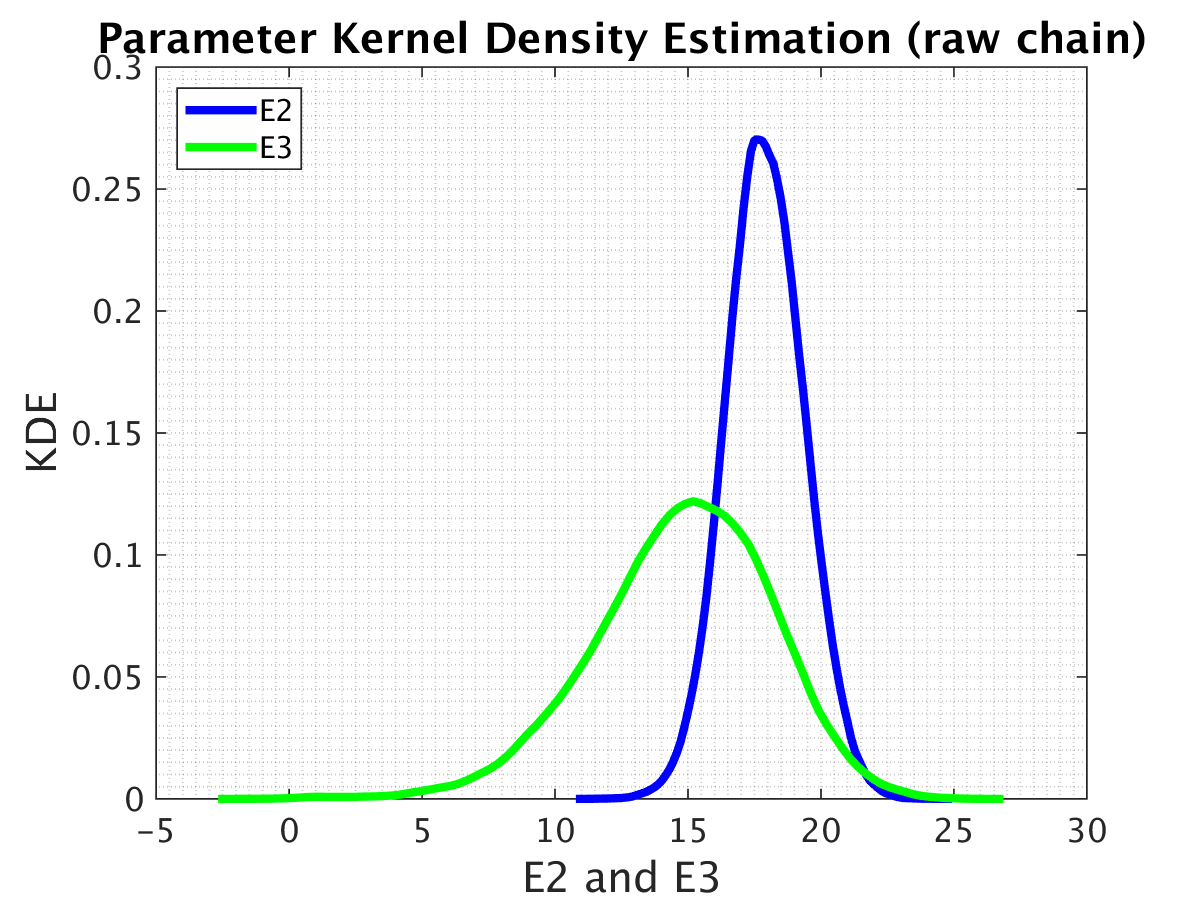
\includegraphics[scale=0.7]{multiple_data/10_kde/outputData_1e6/kde} 
            }  
  \caption{Results for sample size 1e6}
\end{figure}


\begin{figure}[H]
\centering
\subfloat[MCMC raw chain of samples of $E_2$\label{subfig-1:dummy}]{%
     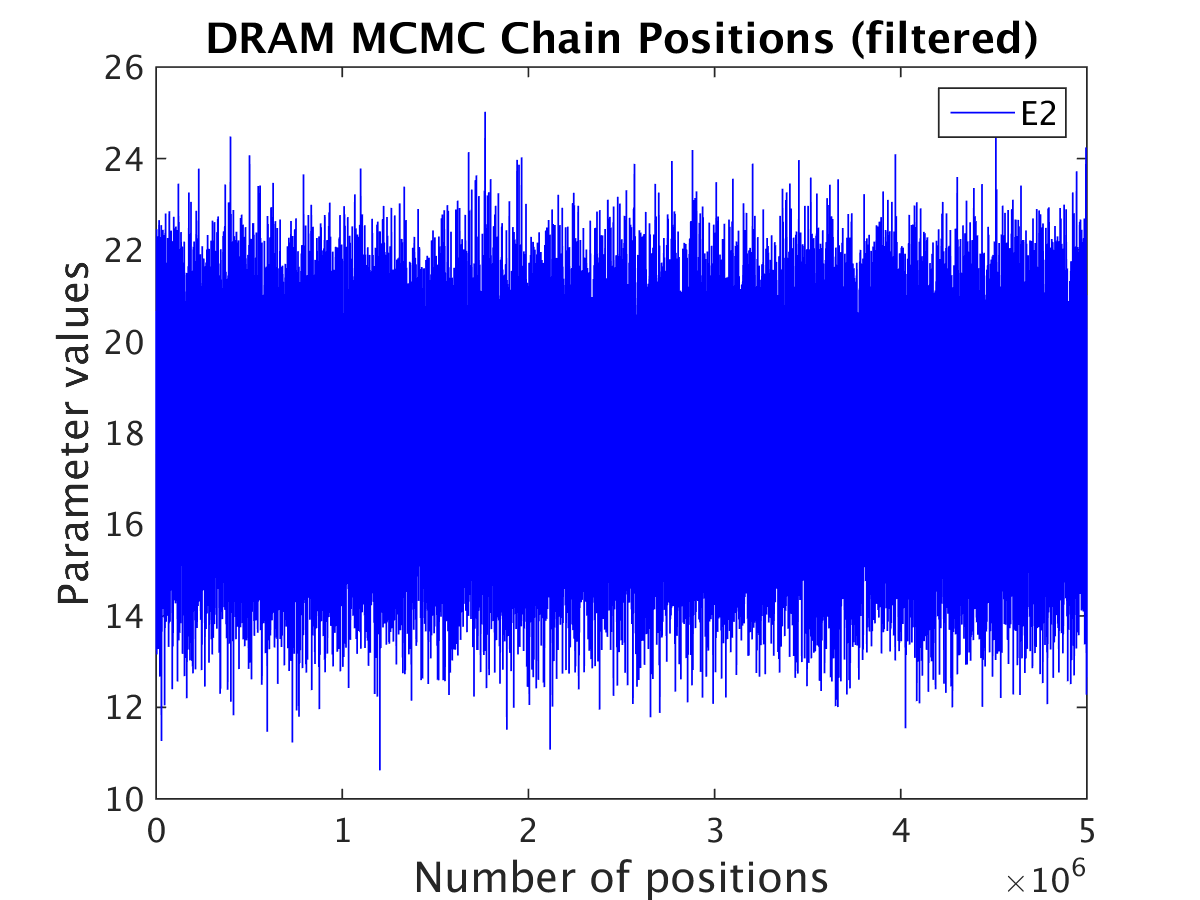
\includegraphics[scale=0.7]{multiple_data/10_kde/outputData_5e6/simple_ip_chain_pos_raw_1} 
    }
    \quad
    \subfloat[MCMC raw chain of samples of $E_2$\label{subfig-1:dummy}]{%
         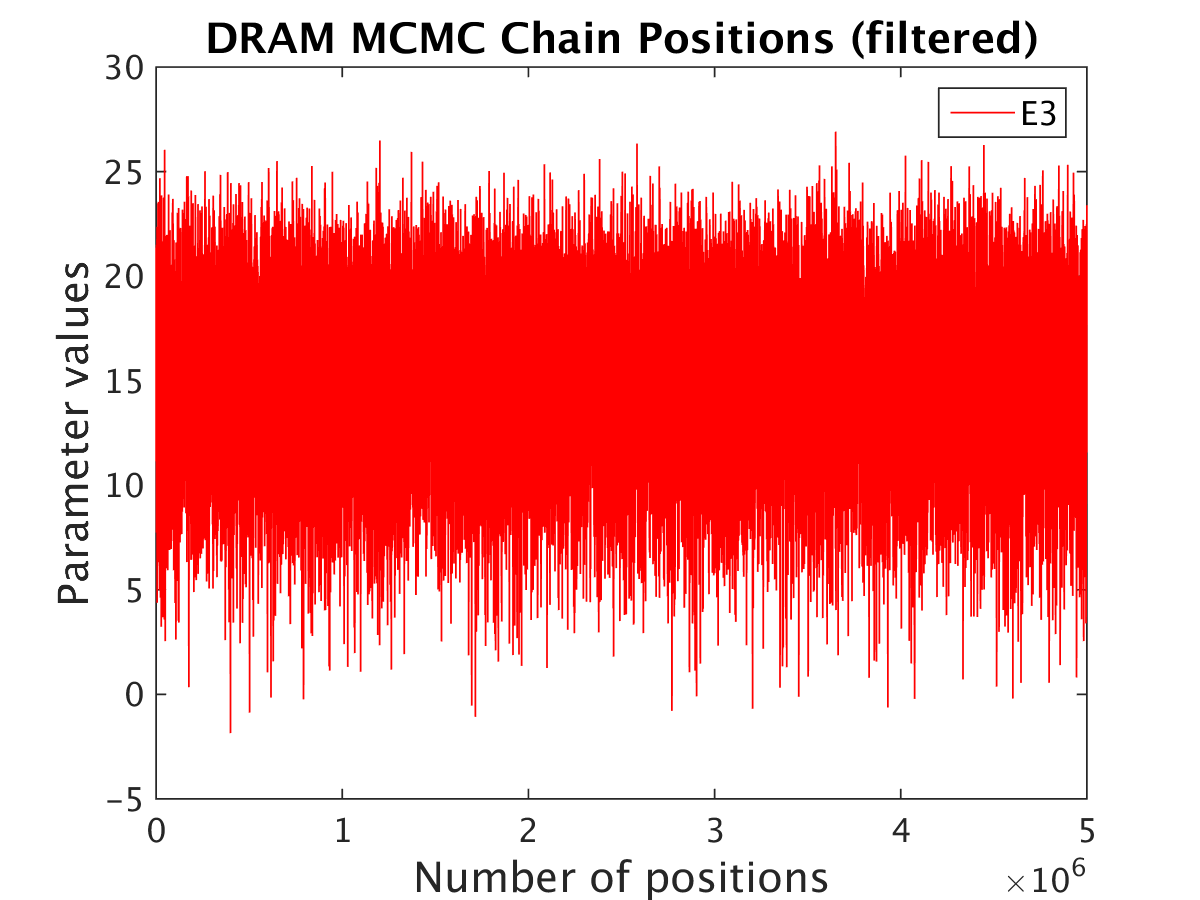
\includegraphics[scale=0.7]{multiple_data/10_kde/outputData_5e6/simple_ip_chain_pos_raw_2} 
        }
    \end{figure}
  \begin{figure}[H]
  \ContinuedFloat
  \centering
  \subfloat[Histogram for $E_2$ \label{subfig-1:dummy}]{%
       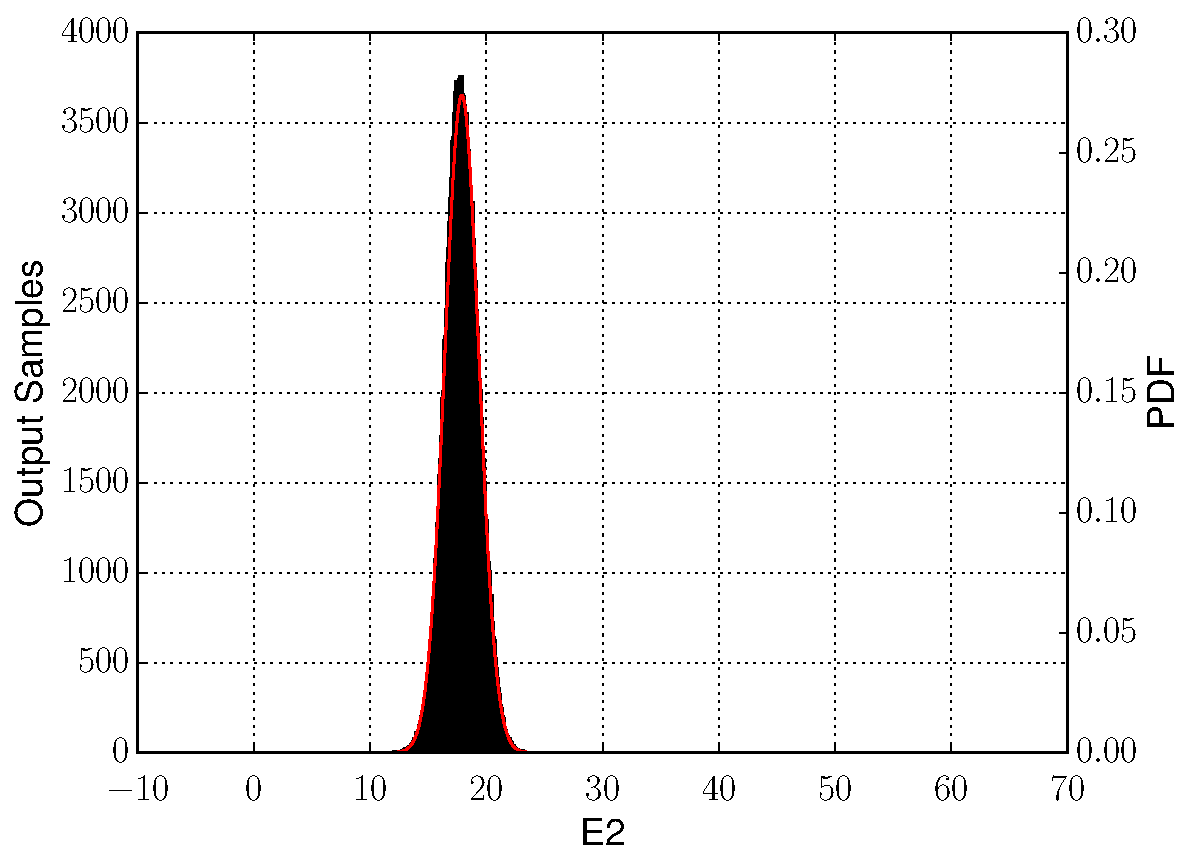
\includegraphics[scale=0.7]{multiple_data/10_kde/outputData_5e6/E2.pdf} 
      }
   \quad
    \subfloat[Histogram for $E_3$ \label{subfig-1:dummy}]{%
          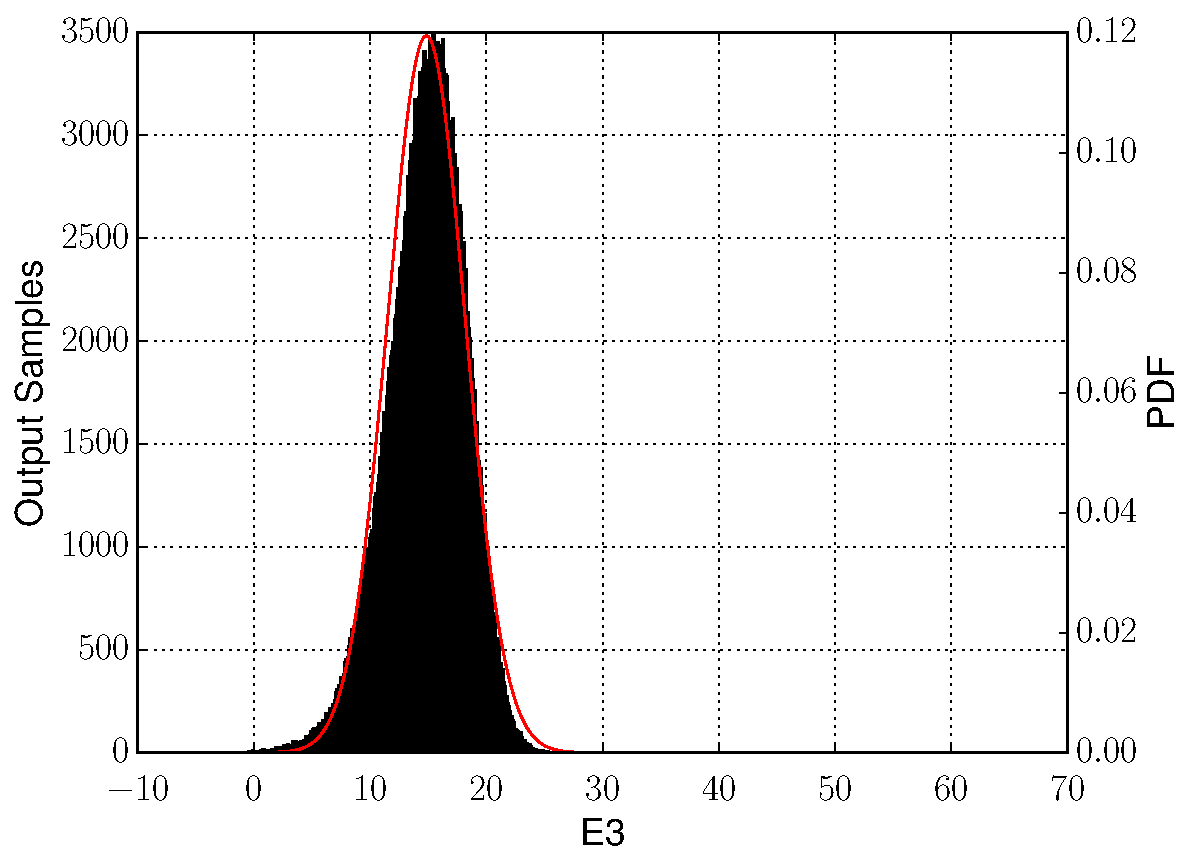
\includegraphics[scale=0.7]{multiple_data/10_kde/outputData_5e6/E3.pdf} 
         }
\end{figure}
\begin{figure}[H]
  
   \subfloat[Cummulative Density Funtion \label{subfig-1:dummy}]{
        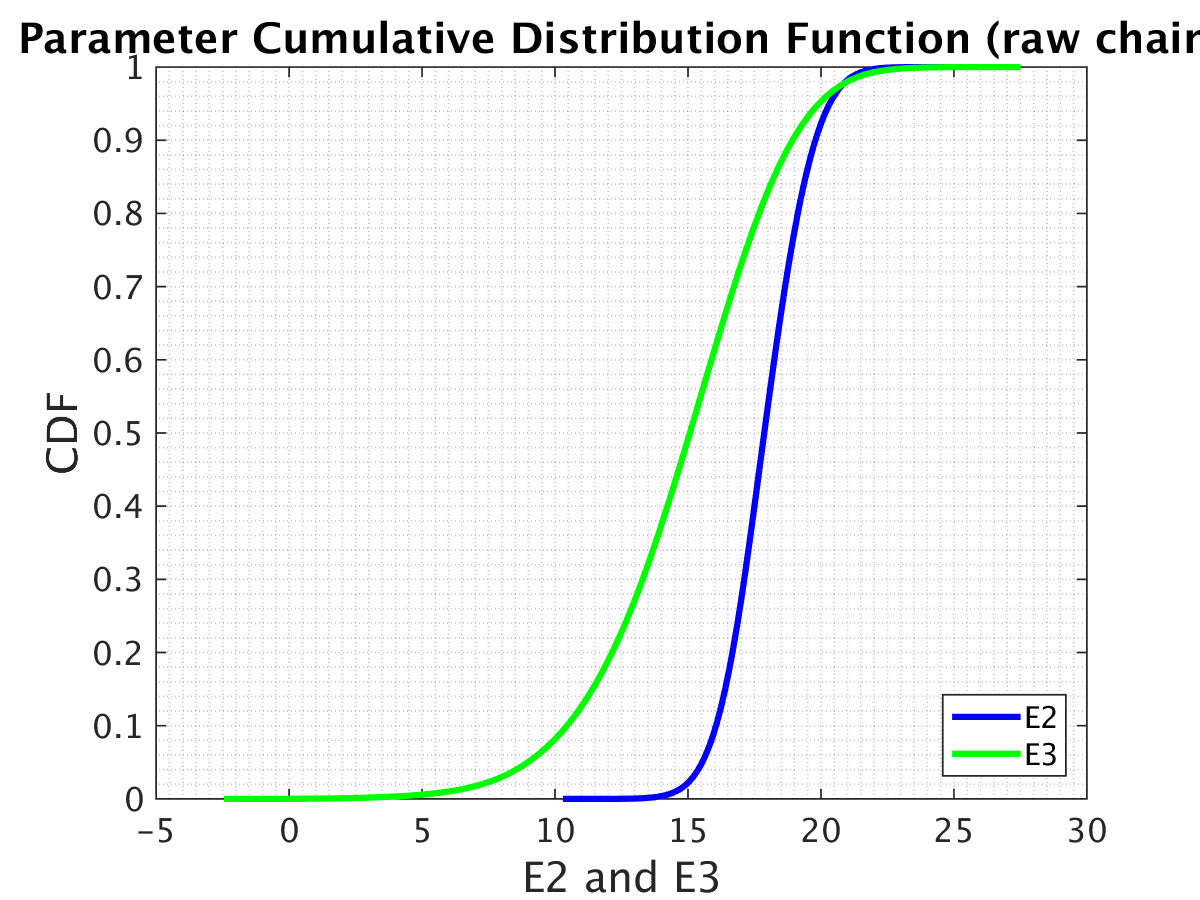
\includegraphics[scale=0.7]{multiple_data/10_kde/outputData_5e6/cdf} 
       }
     \quad
\subfloat[KDE \label{subfig-1:dummy}]{
        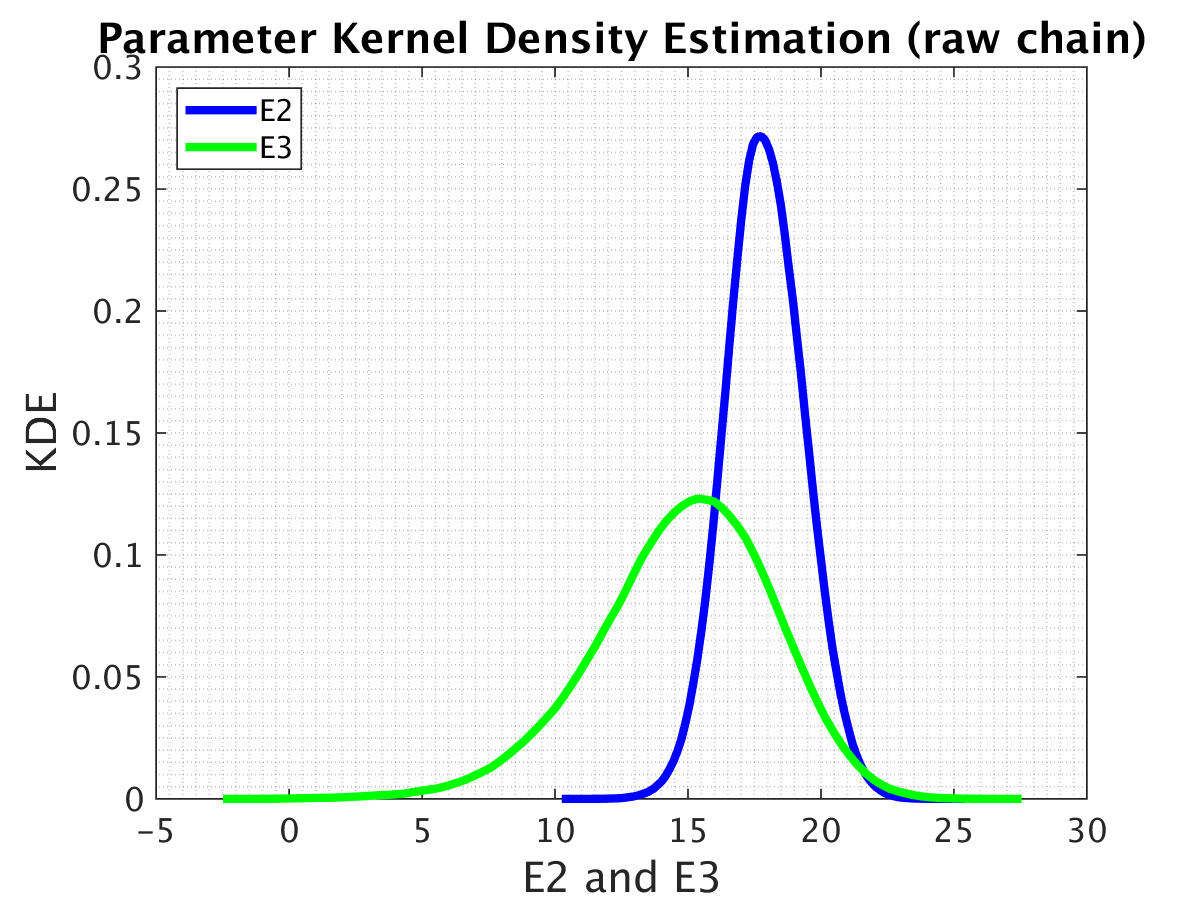
\includegraphics[scale=0.7]{multiple_data/10_kde/outputData_5e6/kde} 
            }  
  \caption{Results for sample size 5e6}
\end{figure}

\begin{figure}[H]
\centering
\subfloat[MCMC raw chain of samples of $E_2$\label{subfig-1:dummy}]{%
     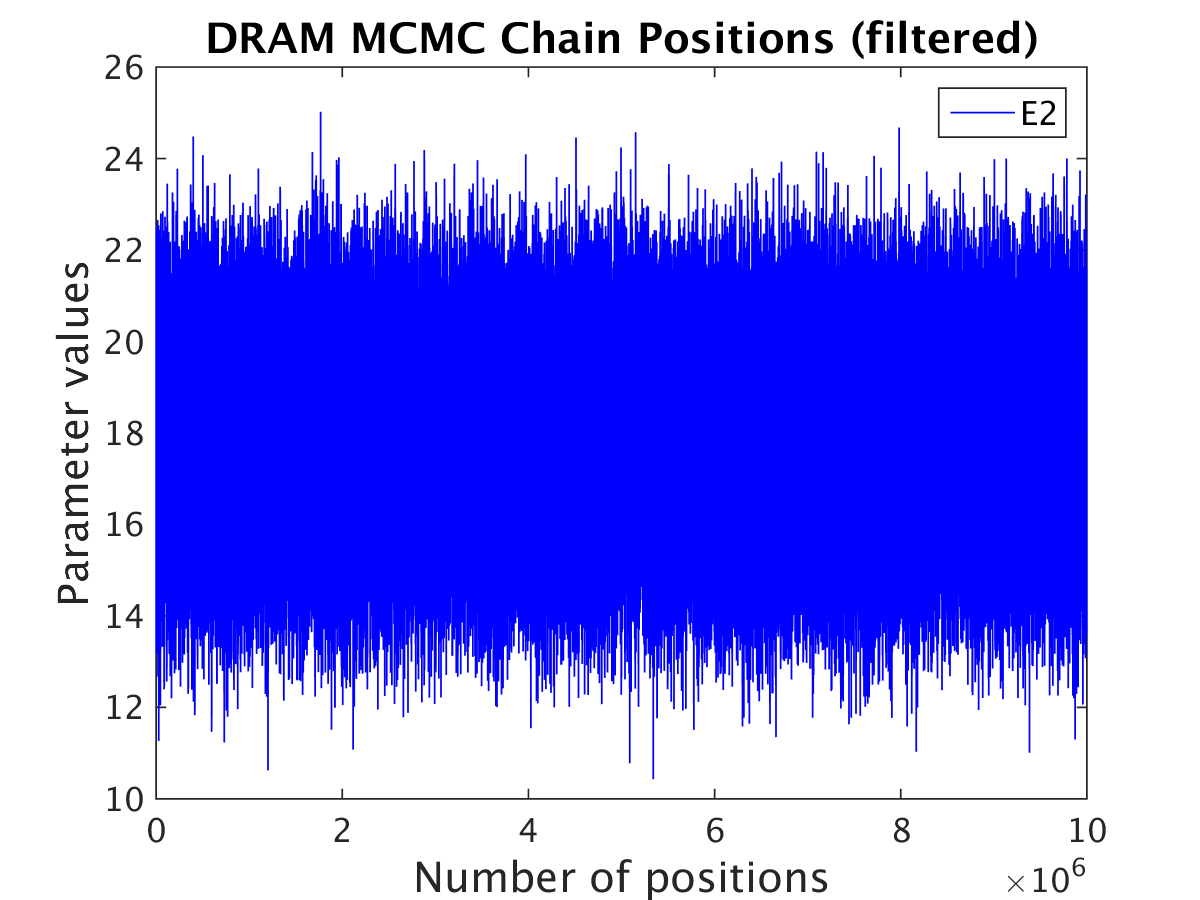
\includegraphics[scale=0.7]{multiple_data/10_kde/outputData_1e7/simple_ip_chain_pos_raw_1} 
    }
    \quad
    \subfloat[MCMC raw chain of samples of $E_2$\label{subfig-1:dummy}]{%
         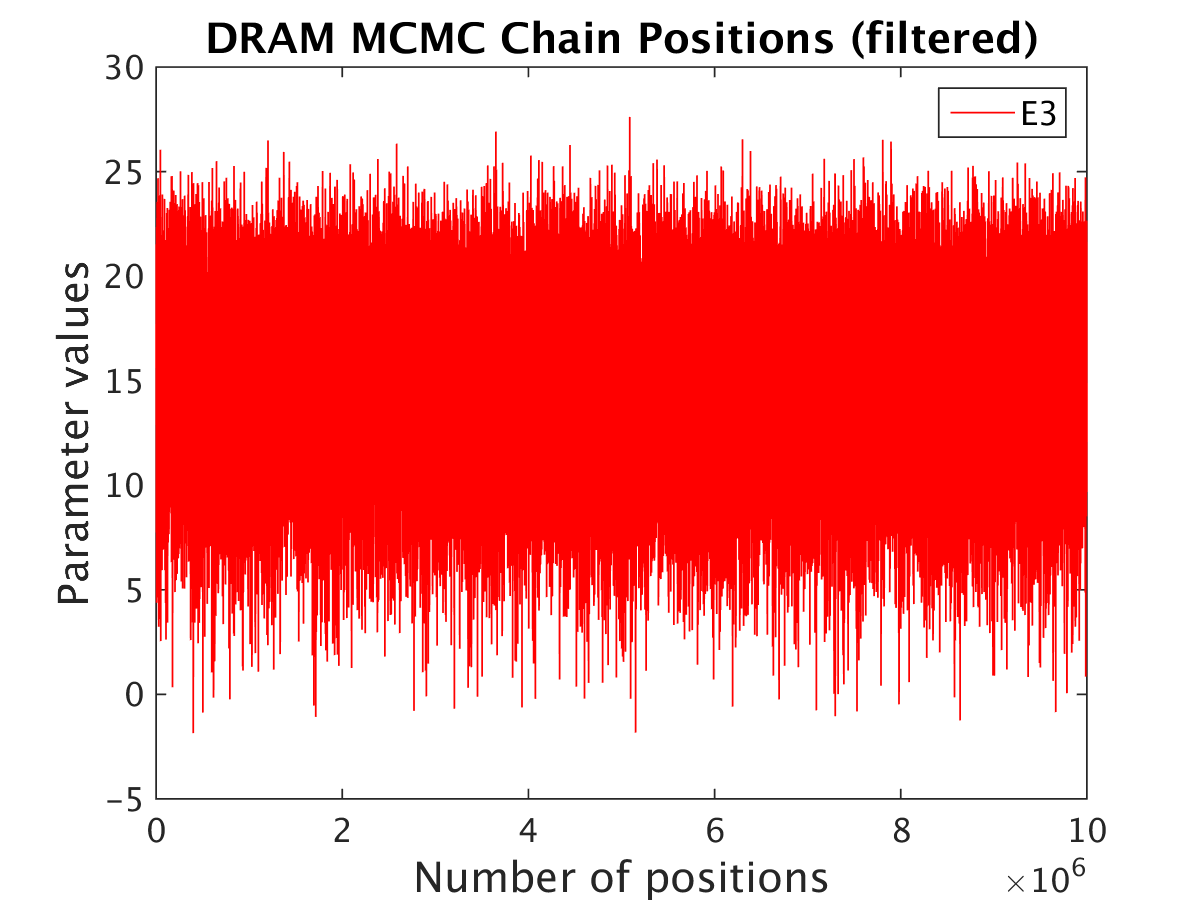
\includegraphics[scale=0.7]{multiple_data/10_kde/outputData_1e7/simple_ip_chain_pos_raw_2} 
        }
    \end{figure}
  \begin{figure}[H]
  \ContinuedFloat
  \centering
  \subfloat[Histogram for $E_2$ \label{subfig-1:dummy}]{%
       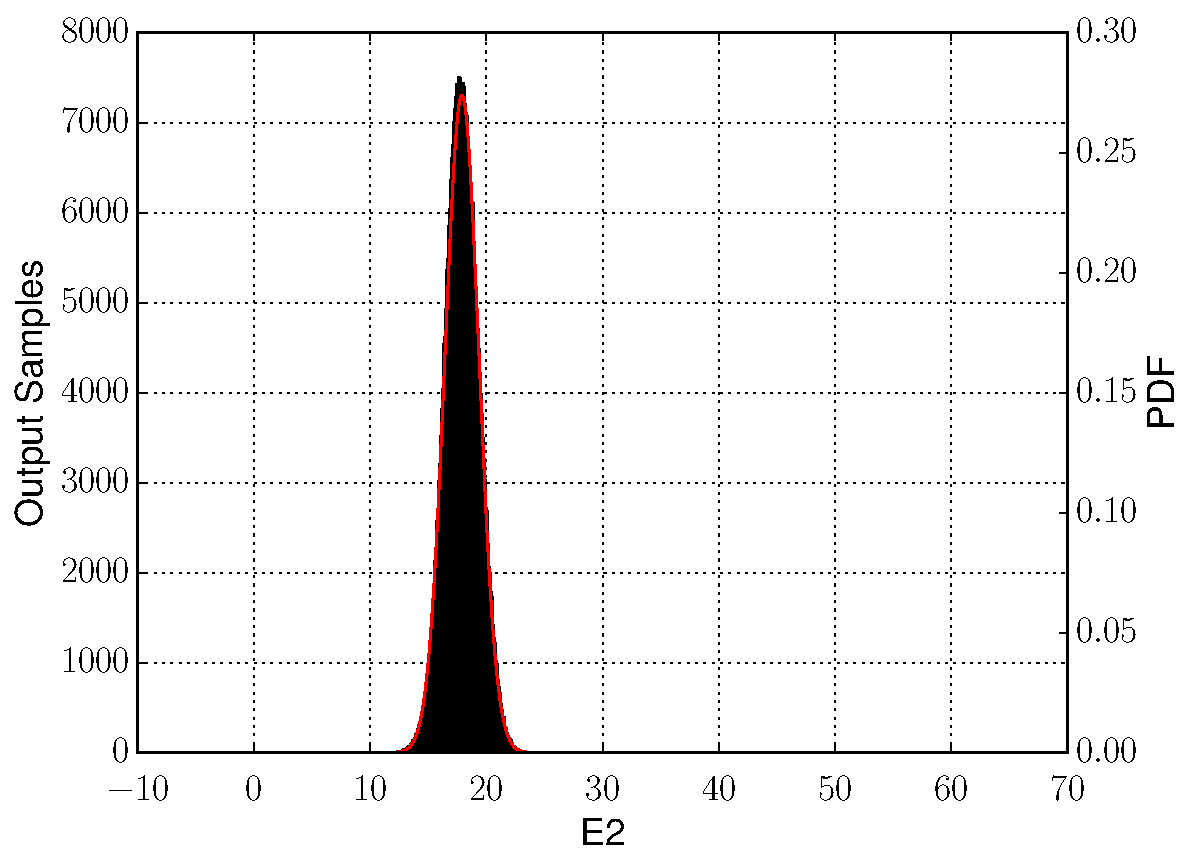
\includegraphics[scale=0.7]{multiple_data/10_kde/outputData_1e7/E2.pdf} 
      }
   \quad
    \subfloat[Histogram for $E_3$ \label{subfig-1:dummy}]{%
          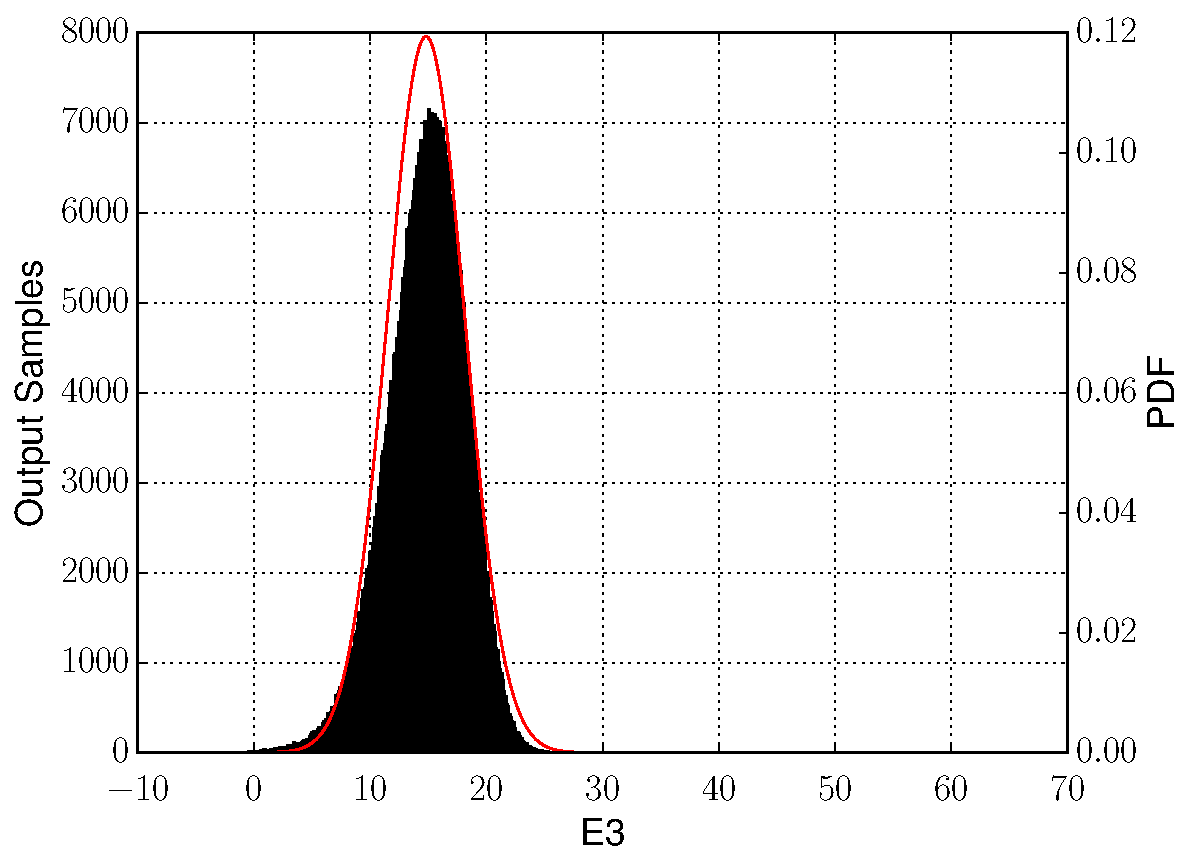
\includegraphics[scale=0.7]{multiple_data/10_kde/outputData_1e7/E3.pdf} 
         }
\end{figure}
\begin{figure}[H]
  
   \subfloat[Cummulative Density Funtion \label{subfig-1:dummy}]{
        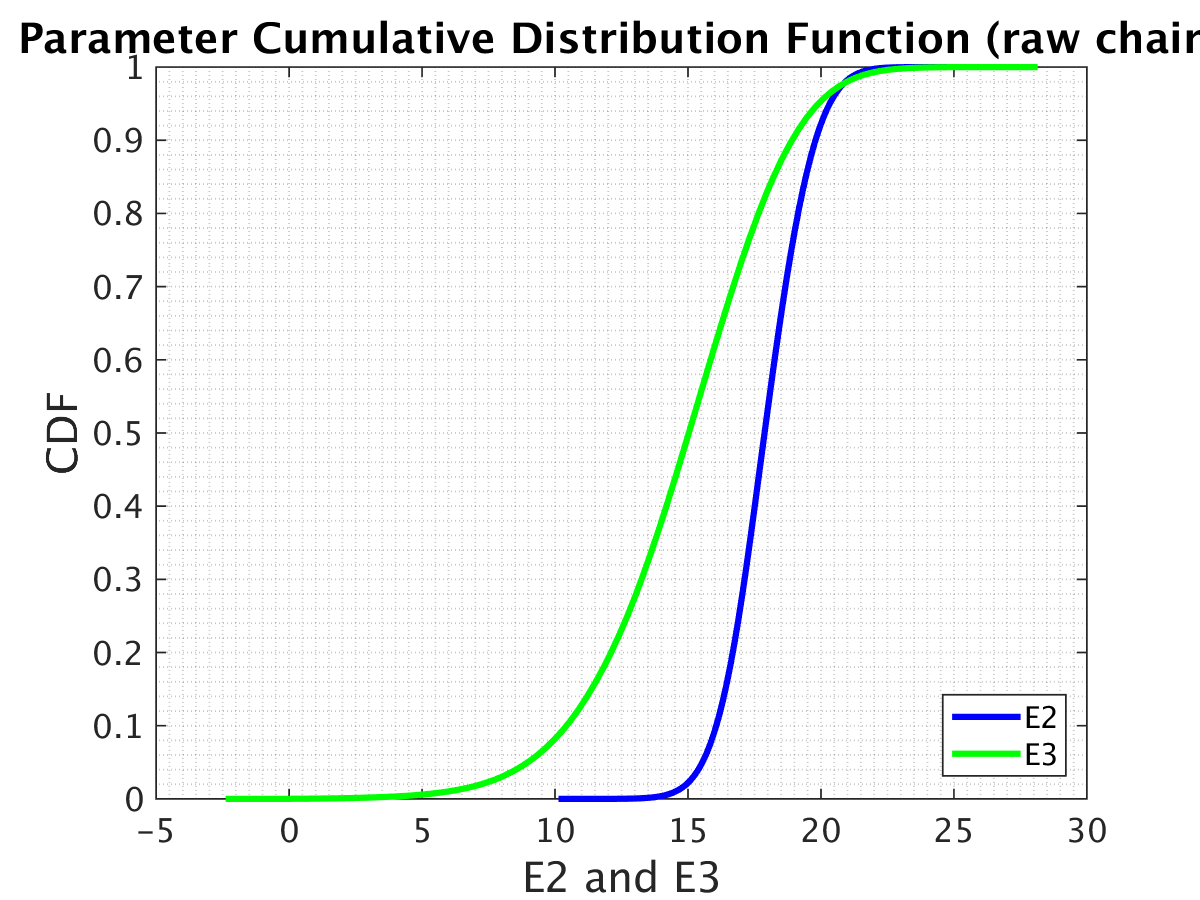
\includegraphics[scale=0.7]{multiple_data/10_kde/outputData_1e7/cdf} 
       }
     \quad
\subfloat[KDE \label{subfig-1:dummy}]{
        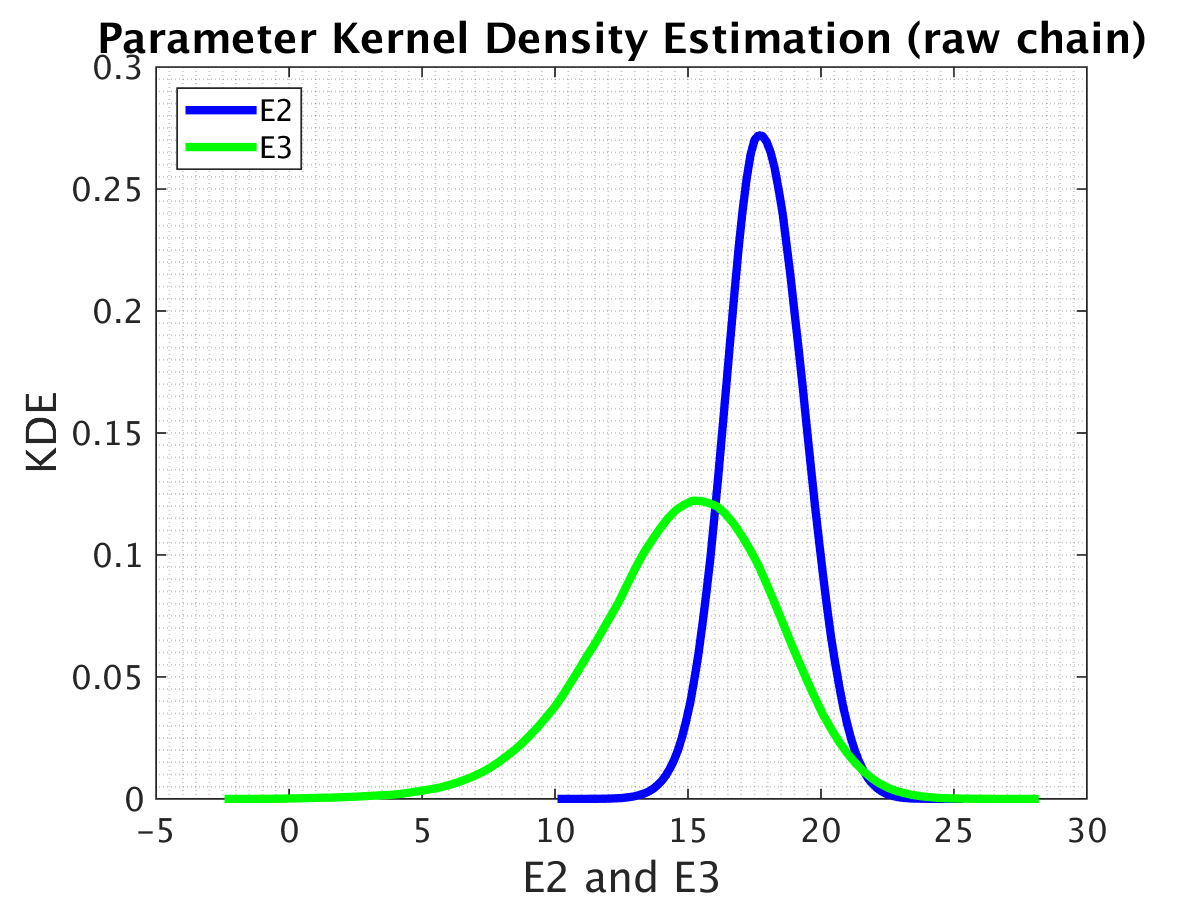
\includegraphics[scale=0.7]{multiple_data/10_kde/outputData_1e7/kde} 
            }  
  \caption{Results for sample size 1e7}
\end{figure}
\subsubsection{Sample size (Surrogate size) 20*20 }
In this section we calculated flamespeed values for 400 (20*20) different points in the domain and the remaining values are linear combination of these 400 points.  The results below are for sample size $1e5$, $5e5$ , $1e6$, $5e6$ and $1e7$. 

\begin{figure}[H]
\centering
\subfloat[MCMC raw chain of samples of $E_2$\label{subfig-1:dummy}]{%
     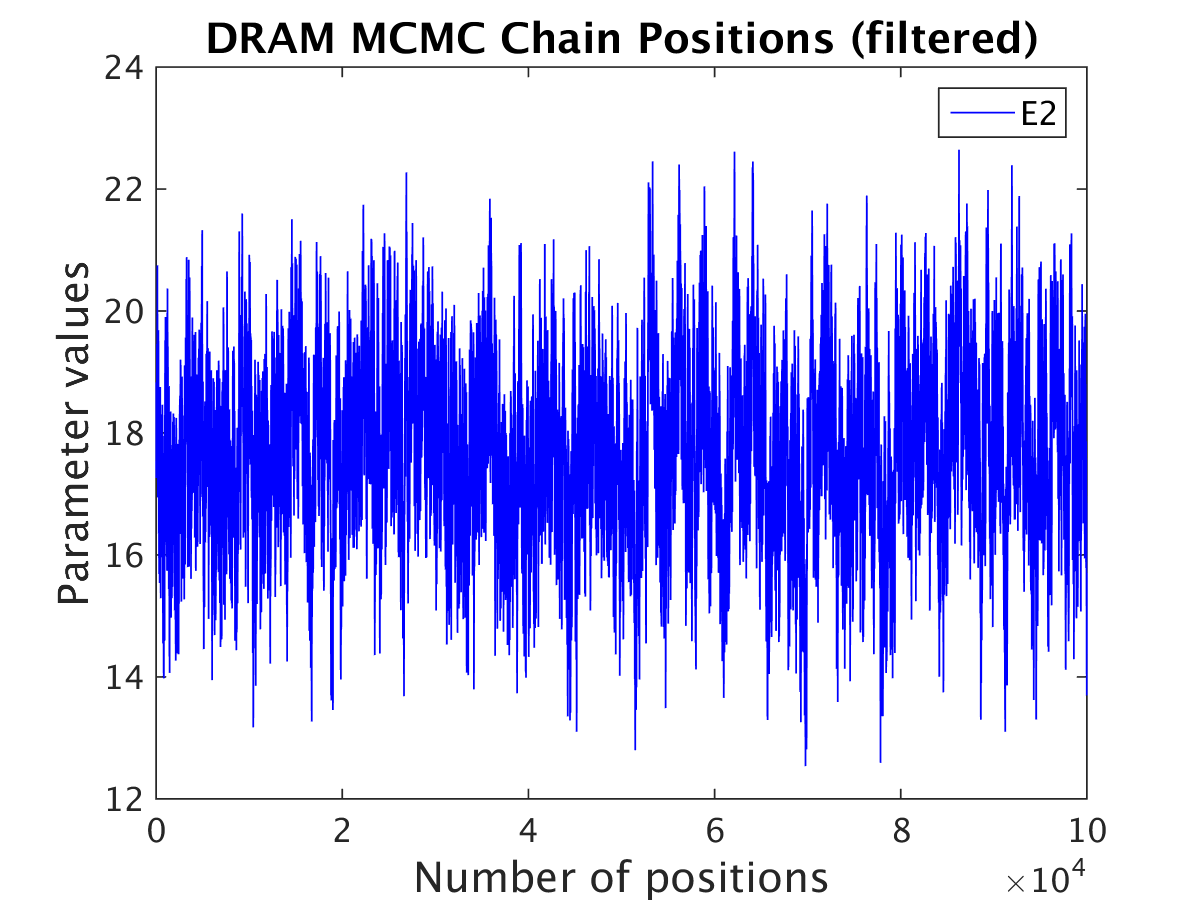
\includegraphics[scale=0.7]{multiple_data/20_kde/outputData_1e5/simple_ip_chain_pos_raw_1} 
    }
    \quad
    \subfloat[MCMC raw chain of samples of $E_2$\label{subfig-1:dummy}]{%
         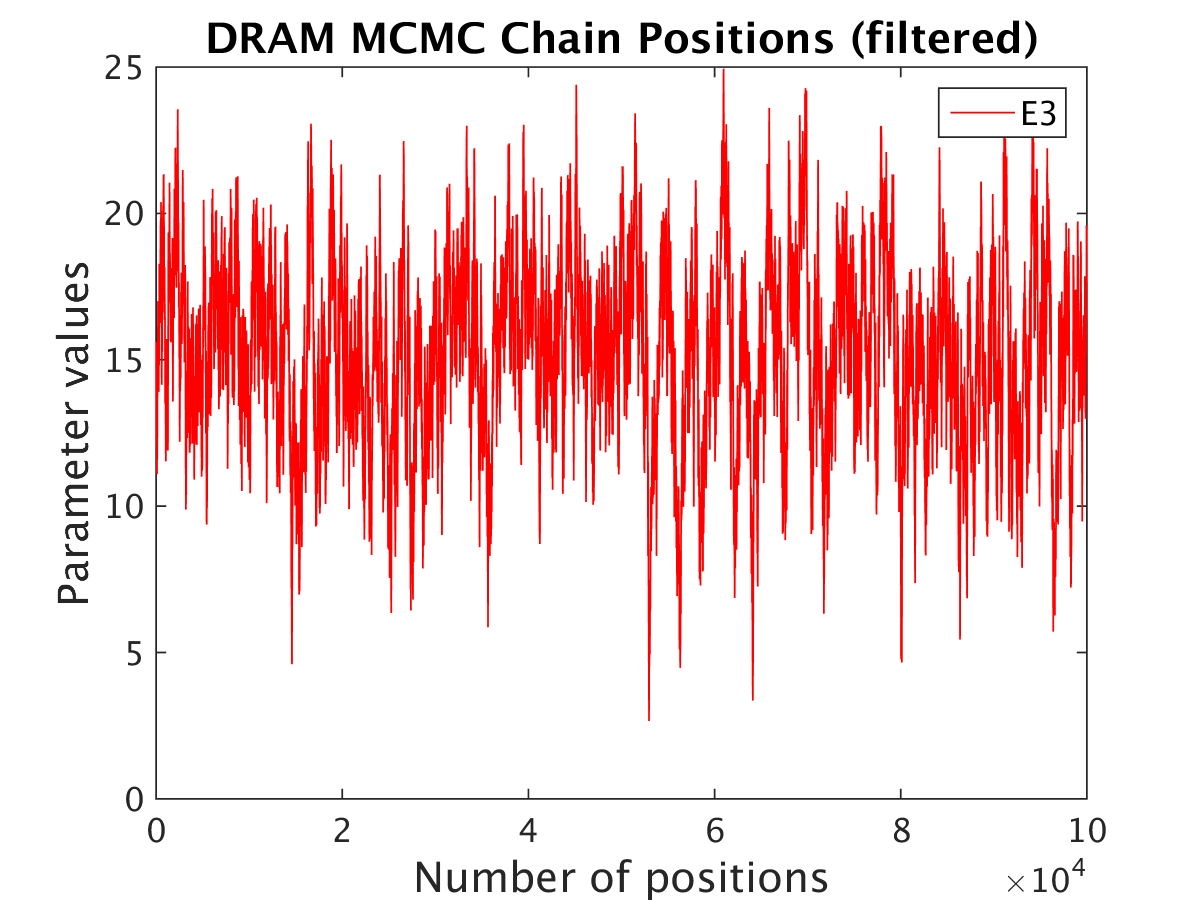
\includegraphics[scale=0.7]{multiple_data/20_kde/outputData_1e5/simple_ip_chain_pos_raw_2} 
        }
    \end{figure}
  \begin{figure}[H]
  \ContinuedFloat
  \centering
  \subfloat[Histogram for $E_2$ \label{subfig-1:dummy}]{%
       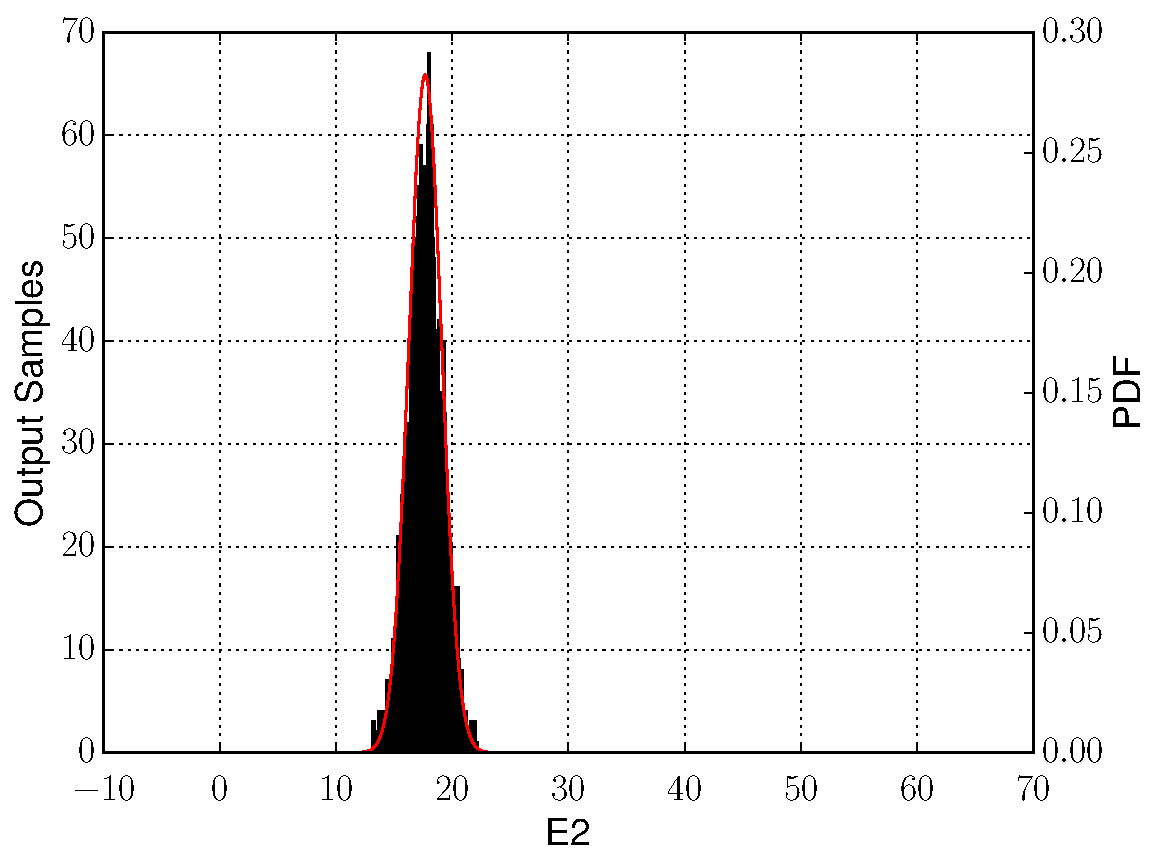
\includegraphics[scale=0.7]{multiple_data/20_kde/outputData_1e5/E2.pdf} 
      }
   \quad
    \subfloat[Histogram for $E_3$ \label{subfig-1:dummy}]{%
          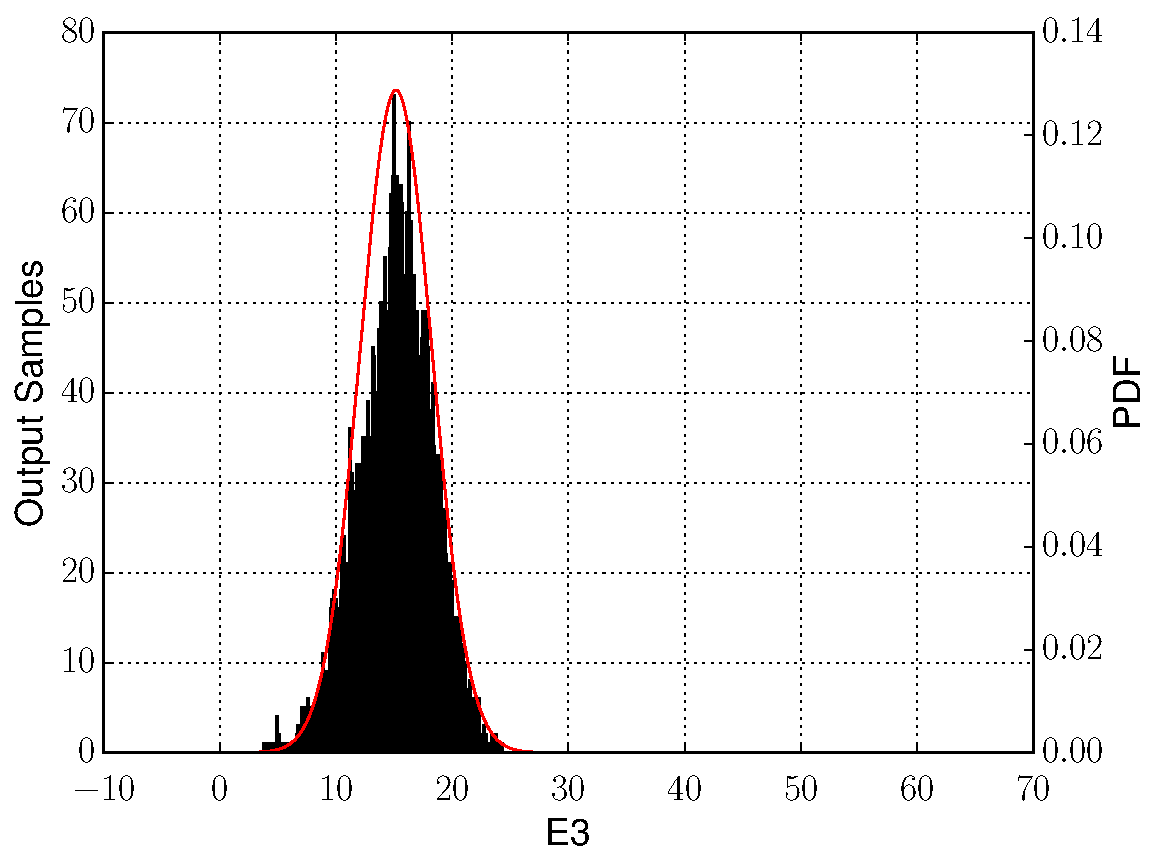
\includegraphics[scale=0.7]{multiple_data/20_kde/outputData_1e5/E3.pdf} 
         }
\end{figure}
\begin{figure}[H]
  
   \subfloat[Cummulative Density Funtion \label{subfig-1:dummy}]{
        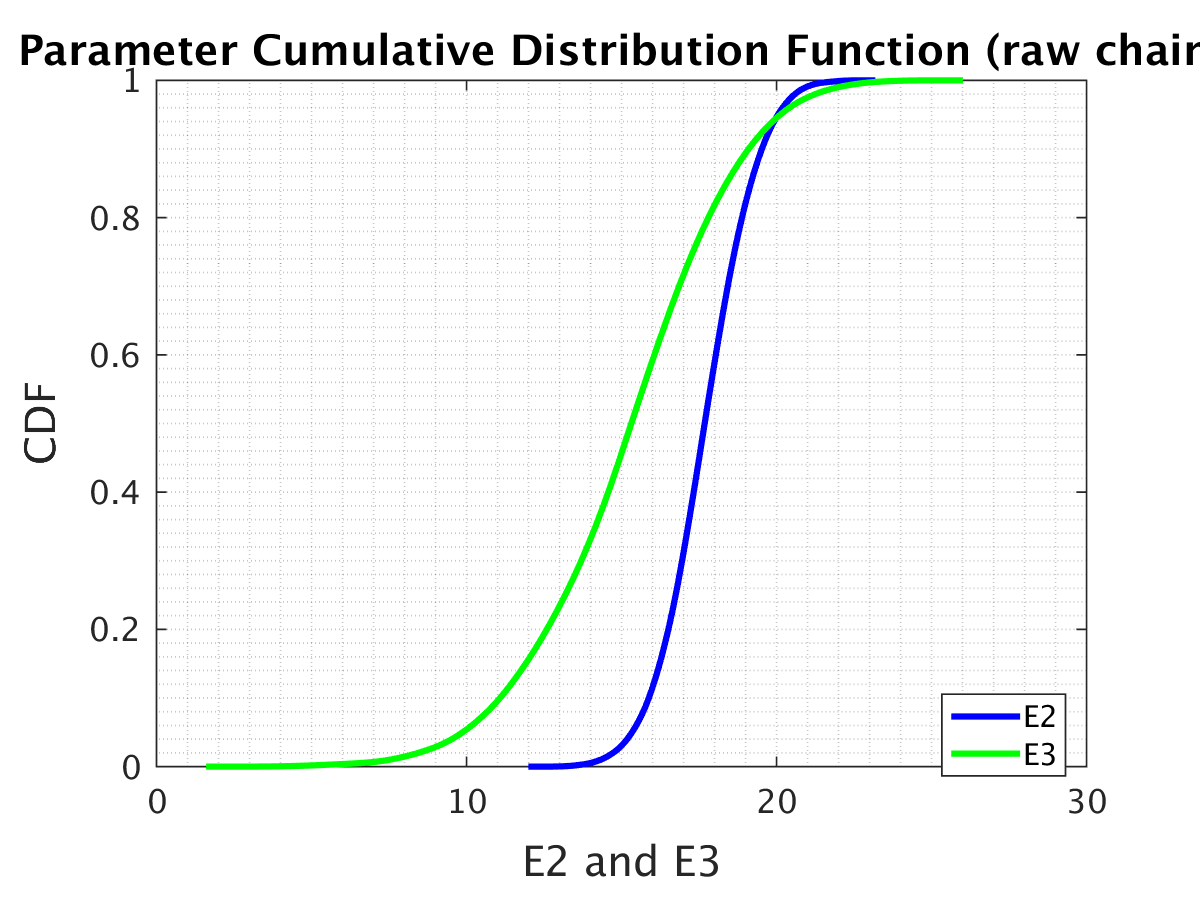
\includegraphics[scale=0.7]{multiple_data/20_kde/outputData_1e5/cdf} 
       }
     \quad
\subfloat[KDE \label{subfig-1:dummy}]{
        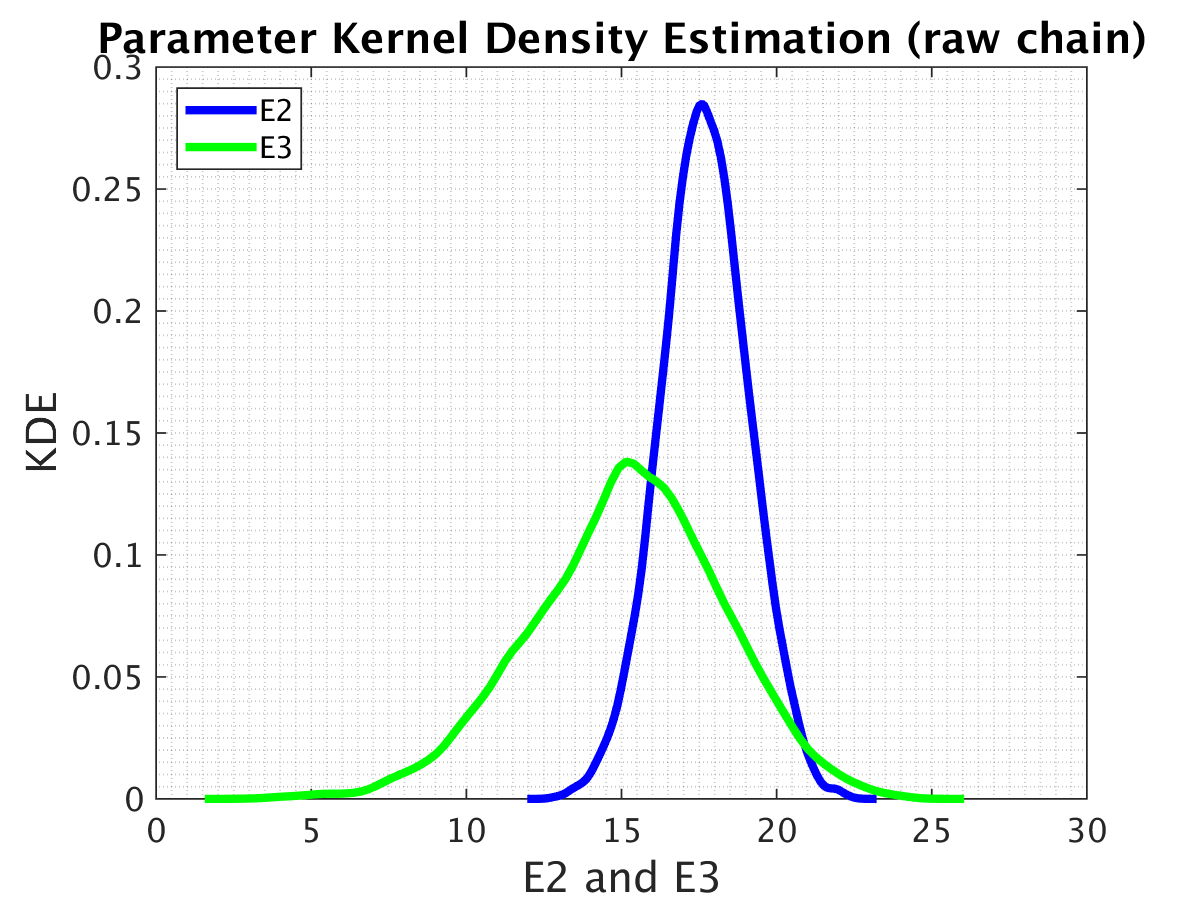
\includegraphics[scale=0.7]{multiple_data/20_kde/outputData_1e5/kde} 
            }  
  \caption{Results for sample size 1e5}
\end{figure}

\begin{figure}[H]
\centering
\subfloat[MCMC raw chain of samples of $E_2$\label{subfig-1:dummy}]{%
     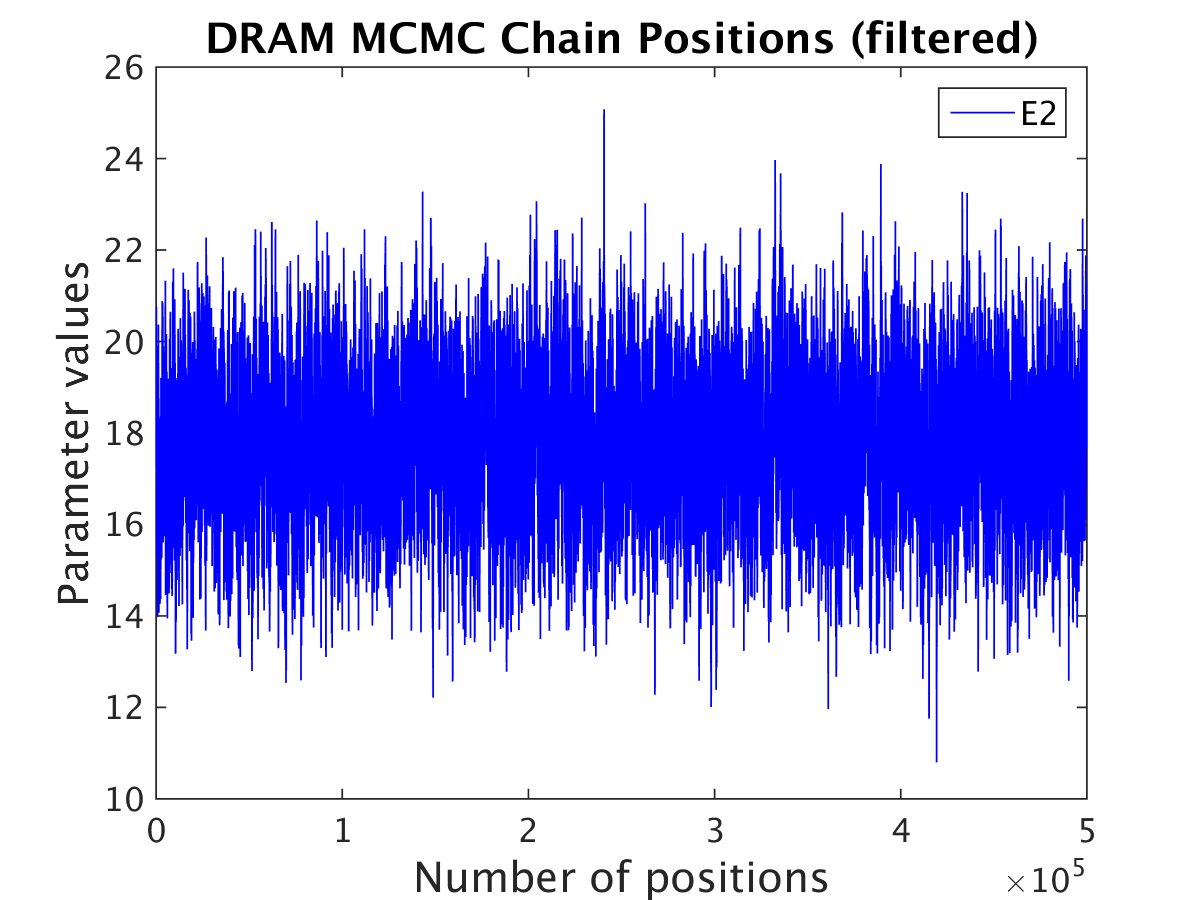
\includegraphics[scale=0.7]{multiple_data/20_kde/outputData_5e5/simple_ip_chain_pos_raw_1} 
    }
    \quad
    \subfloat[MCMC raw chain of samples of $E_2$\label{subfig-1:dummy}]{%
         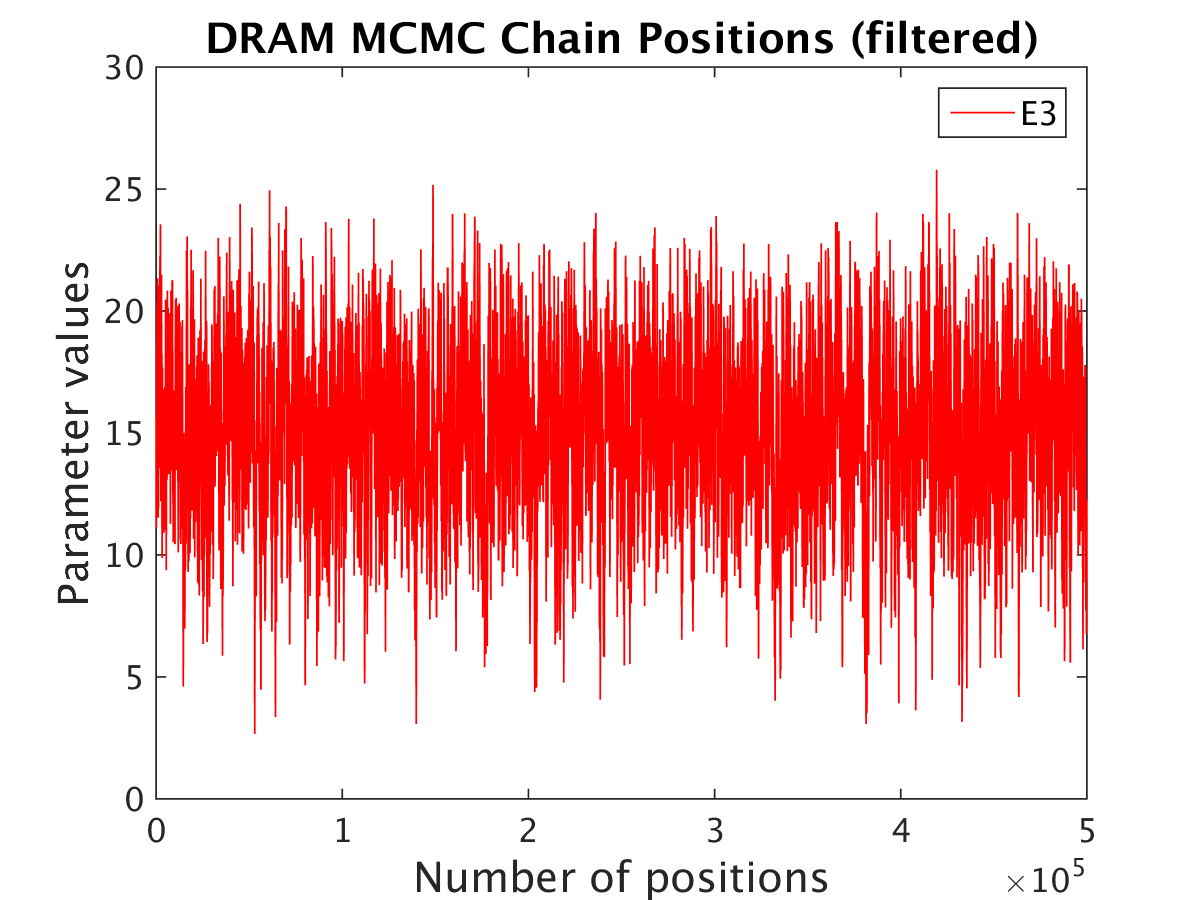
\includegraphics[scale=0.7]{multiple_data/20_kde/outputData_5e5/simple_ip_chain_pos_raw_2} 
        }
    \end{figure}
  \begin{figure}[H]
  \ContinuedFloat
  \centering
  \subfloat[Histogram for $E_2$ \label{subfig-1:dummy}]{%
       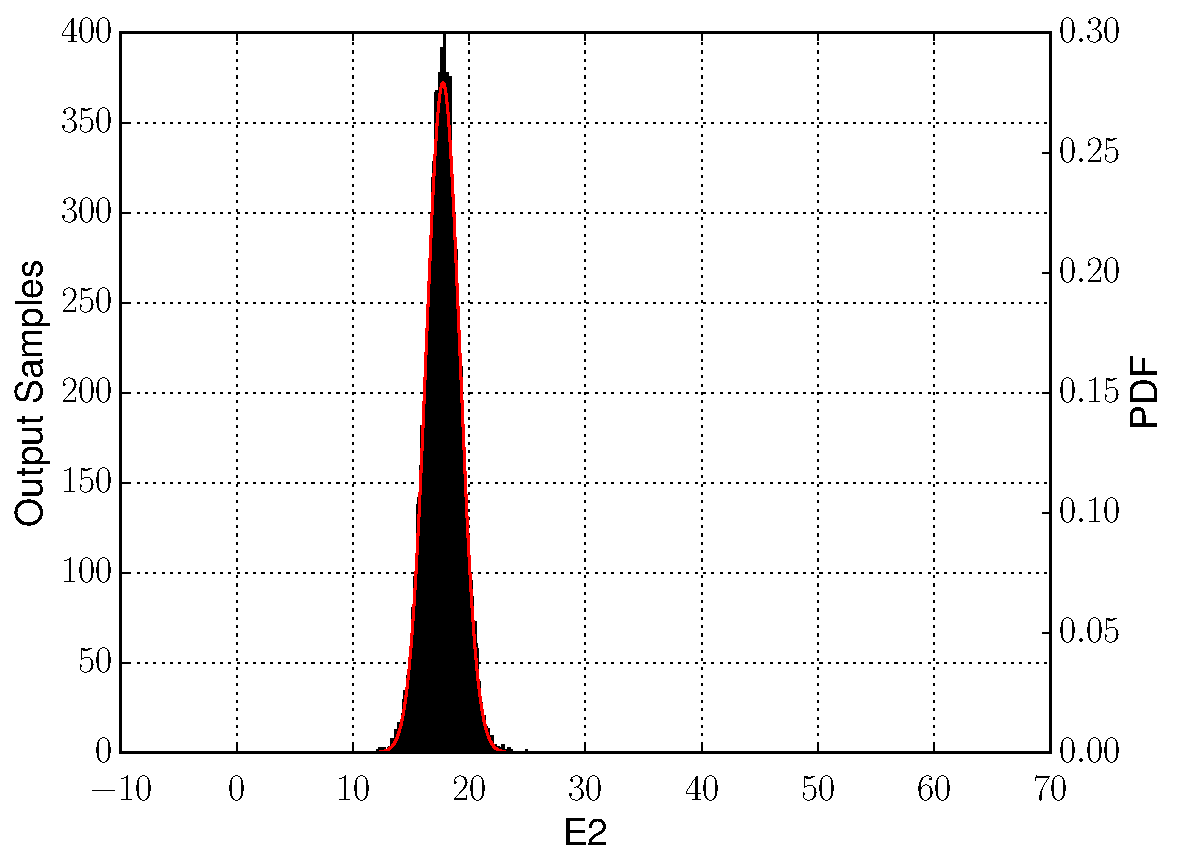
\includegraphics[scale=0.7]{multiple_data/20_kde/outputData_5e5/E2.pdf} 
      }
   \quad
    \subfloat[Histogram for $E_3$ \label{subfig-1:dummy}]{%
          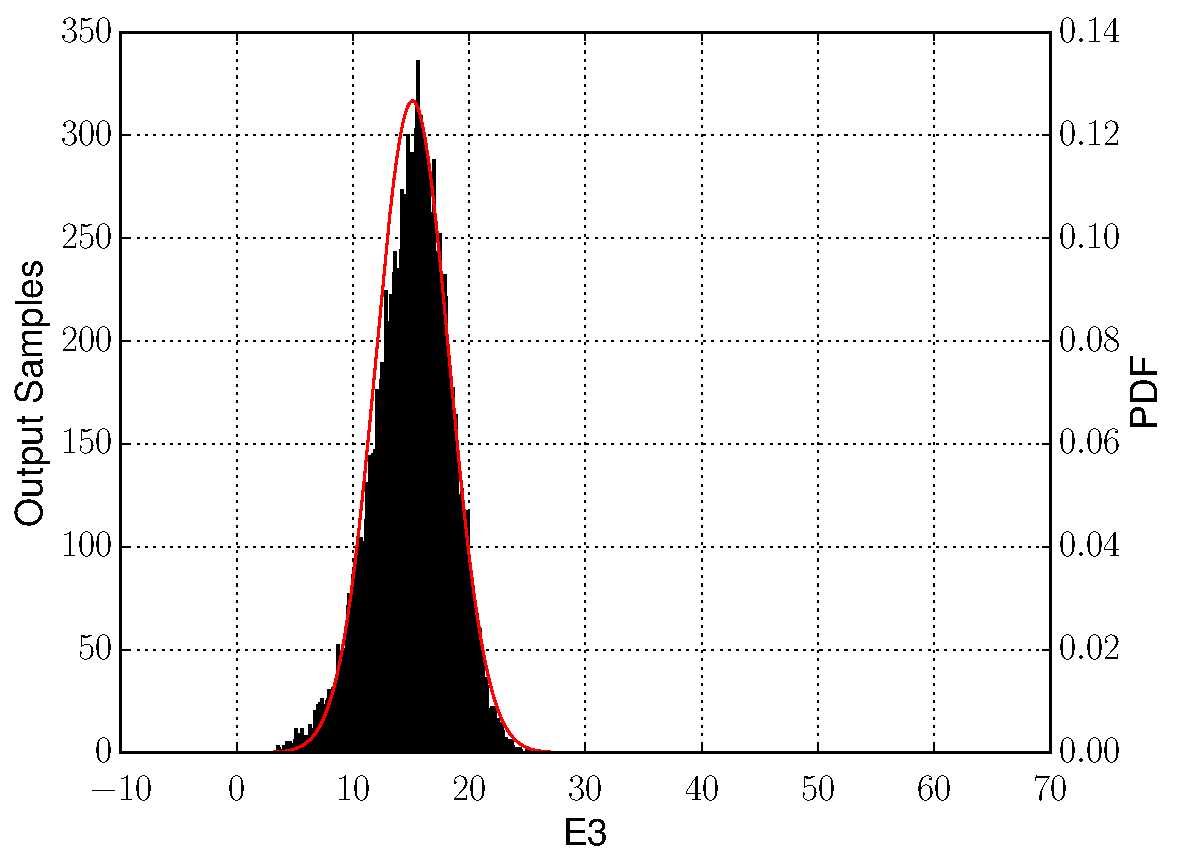
\includegraphics[scale=0.7]{multiple_data/20_kde/outputData_5e5/E3.pdf} 
         }
\end{figure}
\begin{figure}[H]
  
   \subfloat[Cummulative Density Funtion \label{subfig-1:dummy}]{
        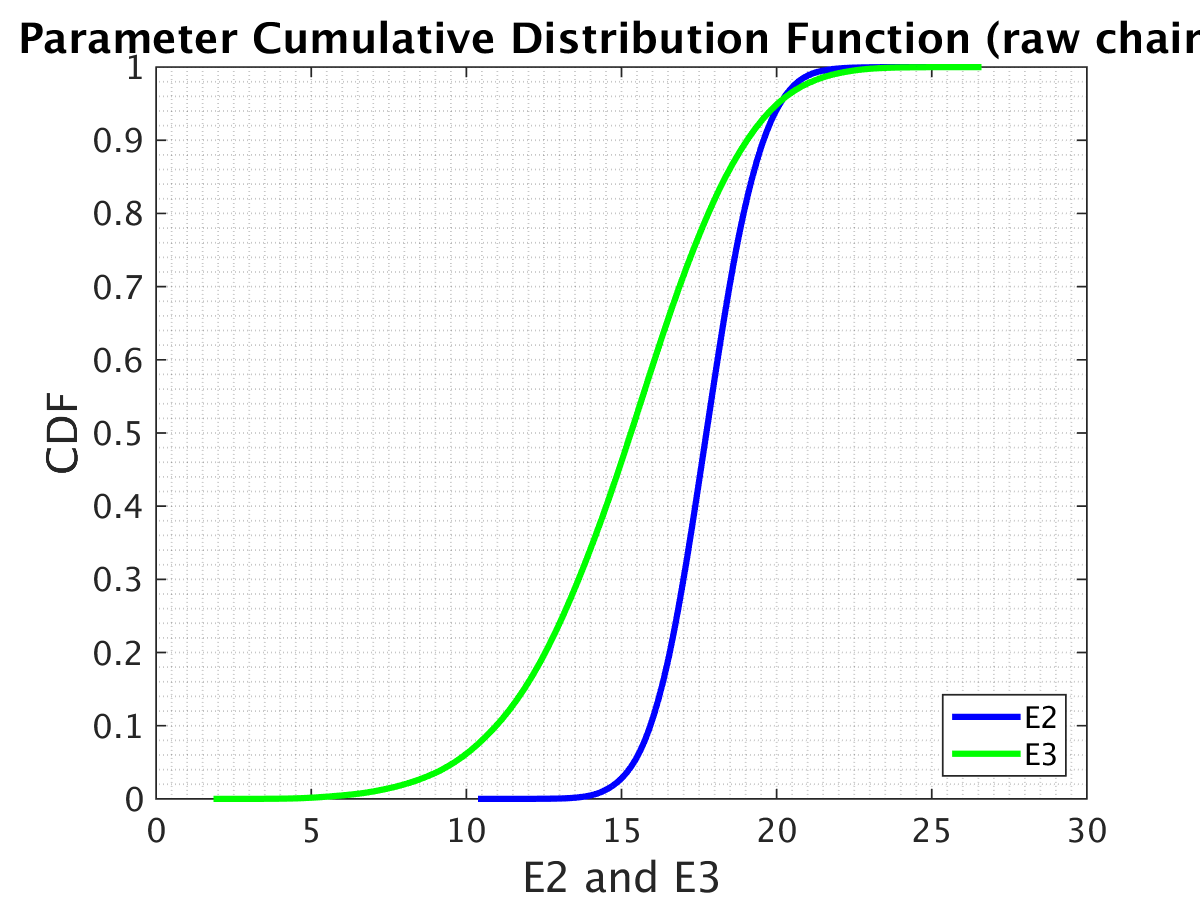
\includegraphics[scale=0.7]{multiple_data/20_kde/outputData_5e5/cdf} 
       }
     \quad
\subfloat[KDE \label{subfig-1:dummy}]{
        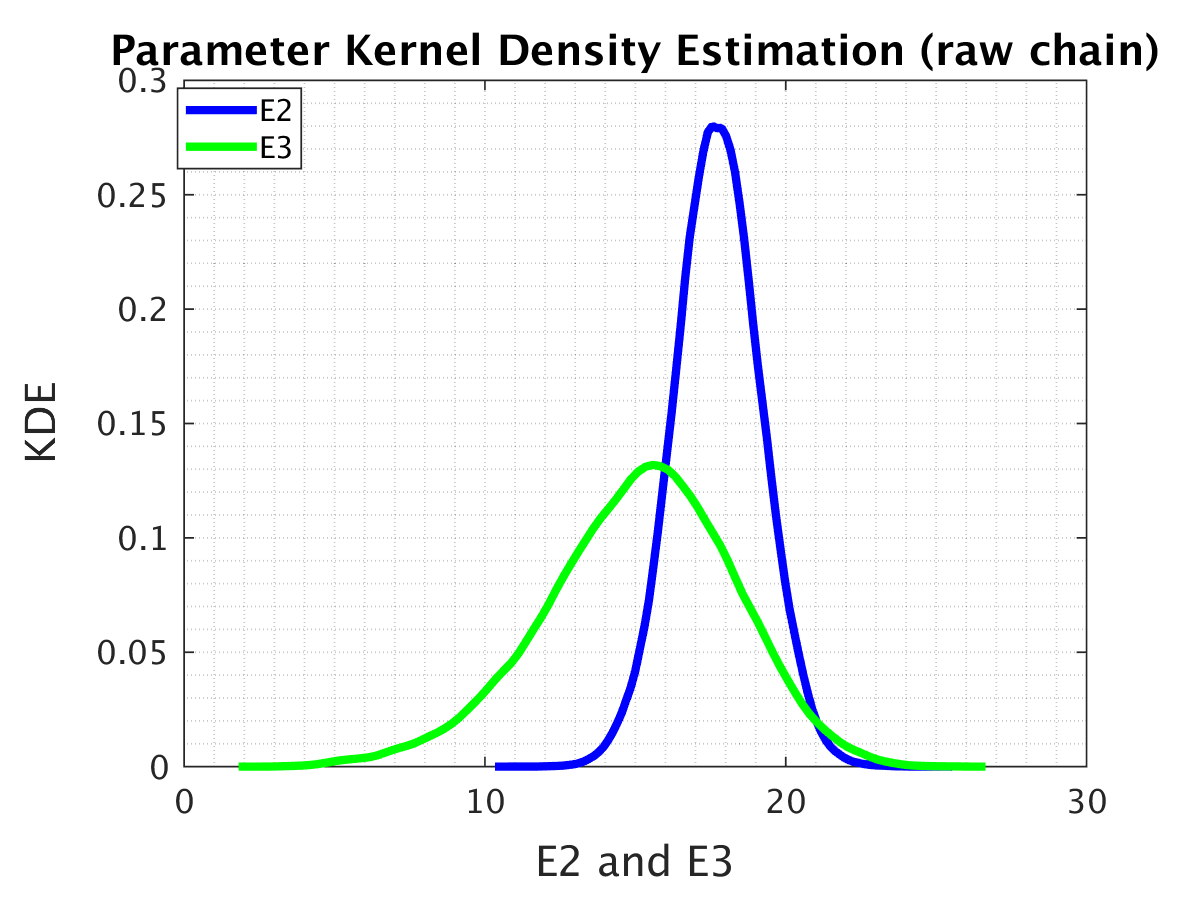
\includegraphics[scale=0.7]{multiple_data/20_kde/outputData_5e5/kde} 
            }  
  \caption{Results for sample size 5e5}
\end{figure}


\begin{figure}[H]
\centering
\subfloat[MCMC raw chain of samples of $E_2$\label{subfig-1:dummy}]{%
     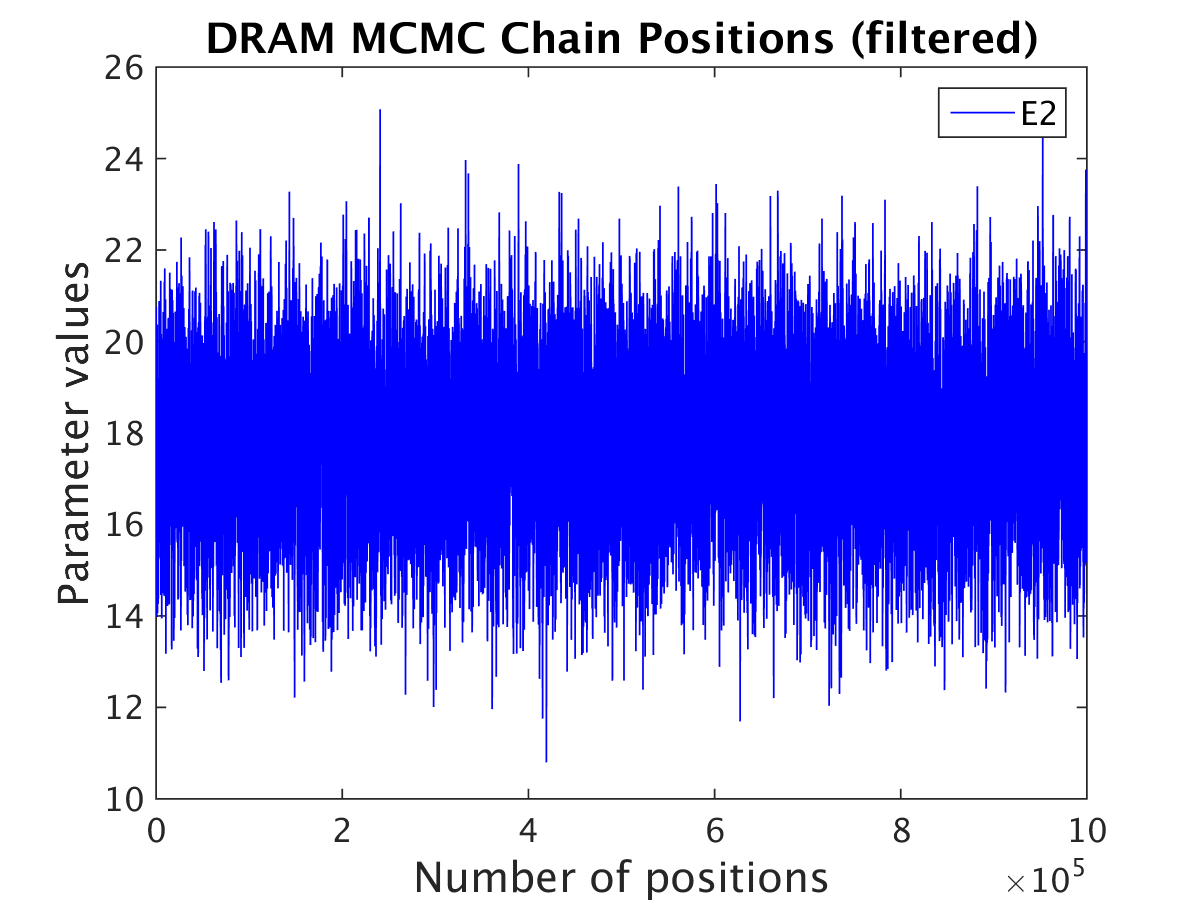
\includegraphics[scale=0.7]{multiple_data/20_kde/outputData_1e6/simple_ip_chain_pos_raw_1} 
    }
    \quad
    \subfloat[MCMC raw chain of samples of $E_2$\label{subfig-1:dummy}]{%
         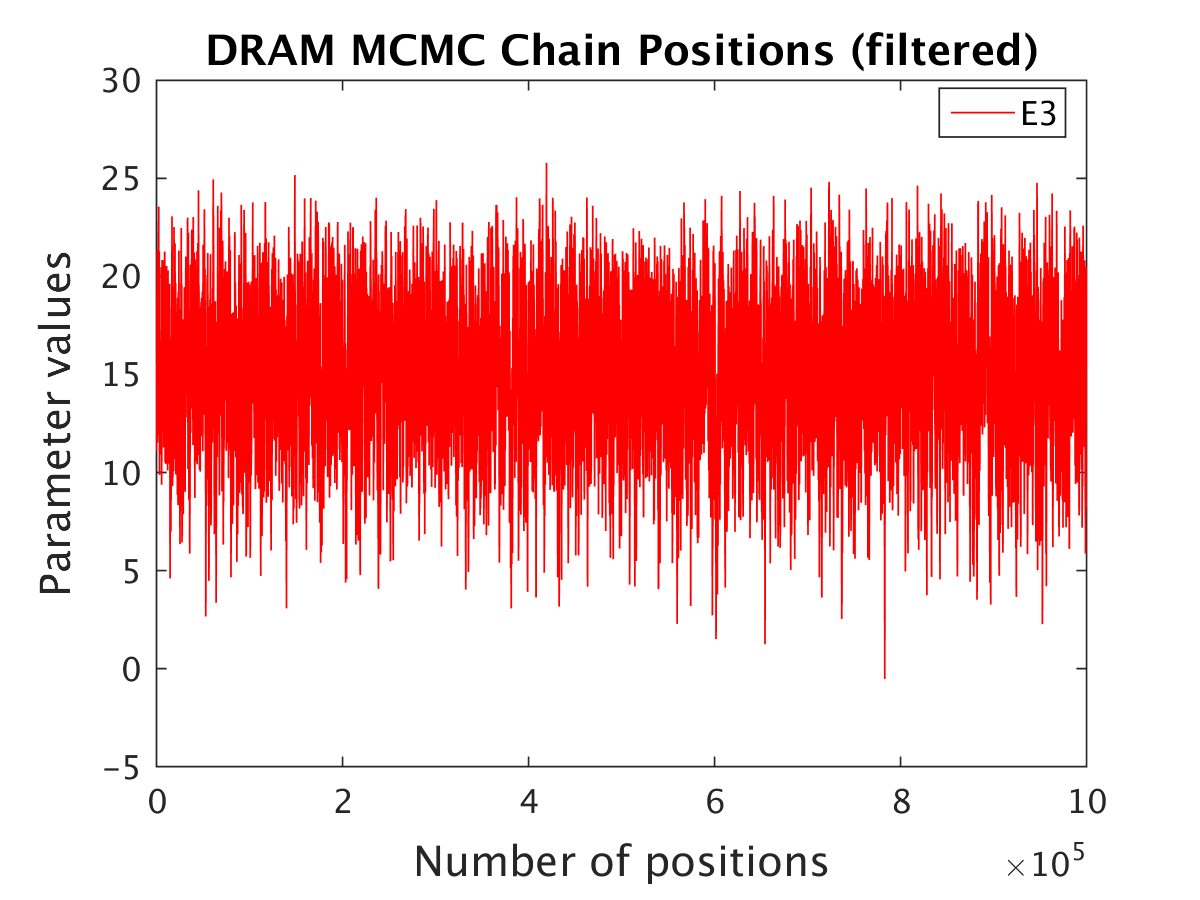
\includegraphics[scale=0.7]{multiple_data/20_kde/outputData_1e6/simple_ip_chain_pos_raw_2} 
        }
    \end{figure}
  \begin{figure}[H]
  \ContinuedFloat
  \centering
  \subfloat[Histogram for $E_2$ \label{subfig-1:dummy}]{%
       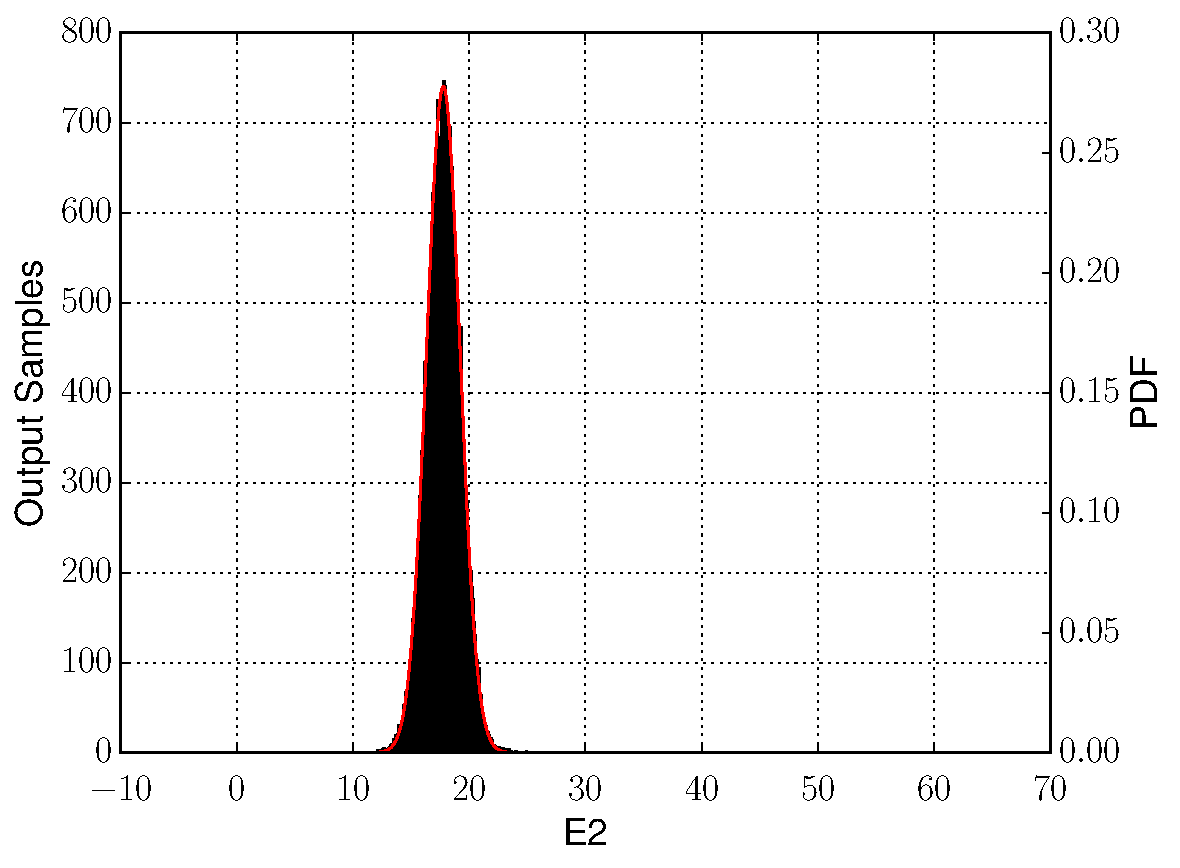
\includegraphics[scale=0.7]{multiple_data/20_kde/outputData_1e6/E2.pdf} 
      }
   \quad
    \subfloat[Histogram for $E_3$ \label{subfig-1:dummy}]{%
          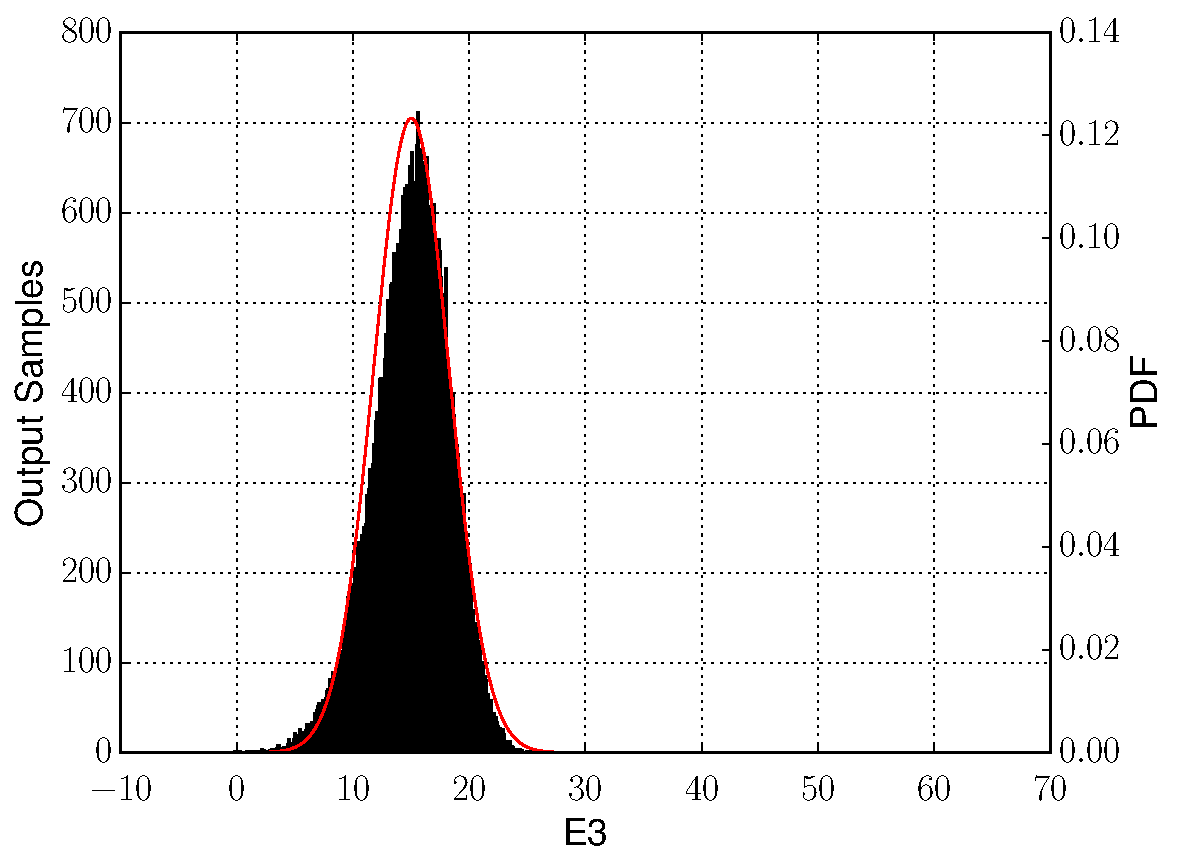
\includegraphics[scale=0.7]{multiple_data/20_kde/outputData_1e6/E3.pdf} 
         }
\end{figure}
\begin{figure}[H]
  
   \subfloat[Cummulative Density Funtion \label{subfig-1:dummy}]{
        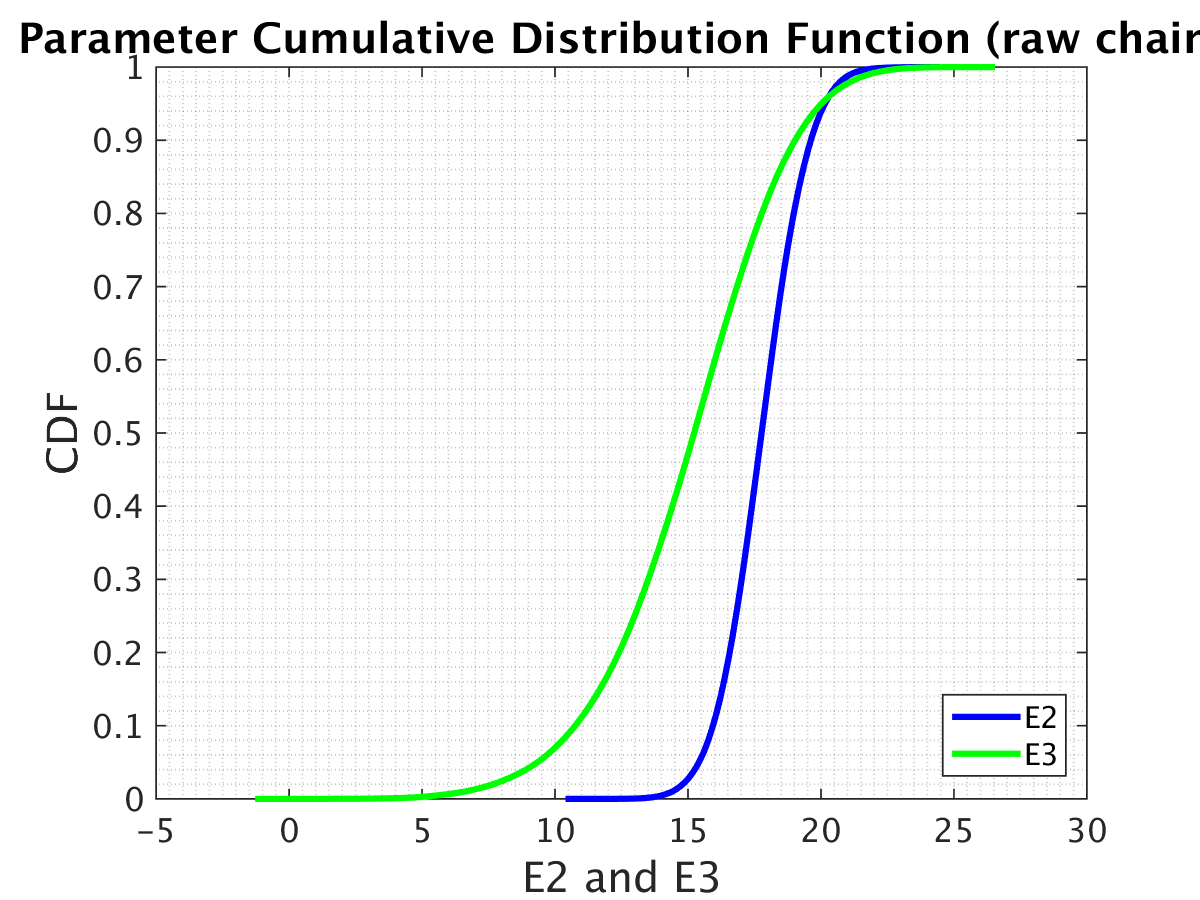
\includegraphics[scale=0.7]{multiple_data/20_kde/outputData_1e6/cdf} 
       }
     \quad
\subfloat[KDE \label{subfig-1:dummy}]{
        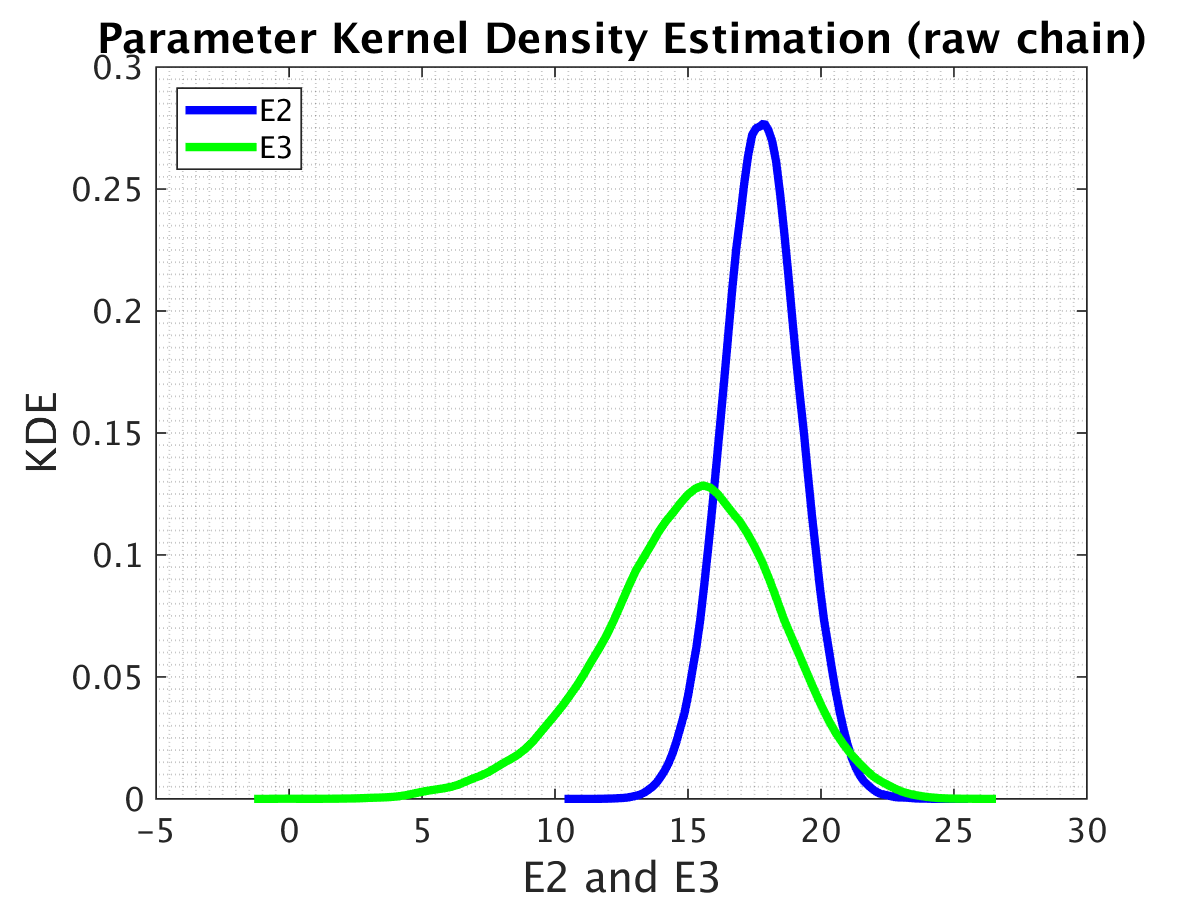
\includegraphics[scale=0.7]{multiple_data/20_kde/outputData_1e6/kde} 
            }  
  \caption{Results for sample size 1e6}
\end{figure}


\begin{figure}[H]
\centering
\subfloat[MCMC raw chain of samples of $E_2$\label{subfig-1:dummy}]{%
     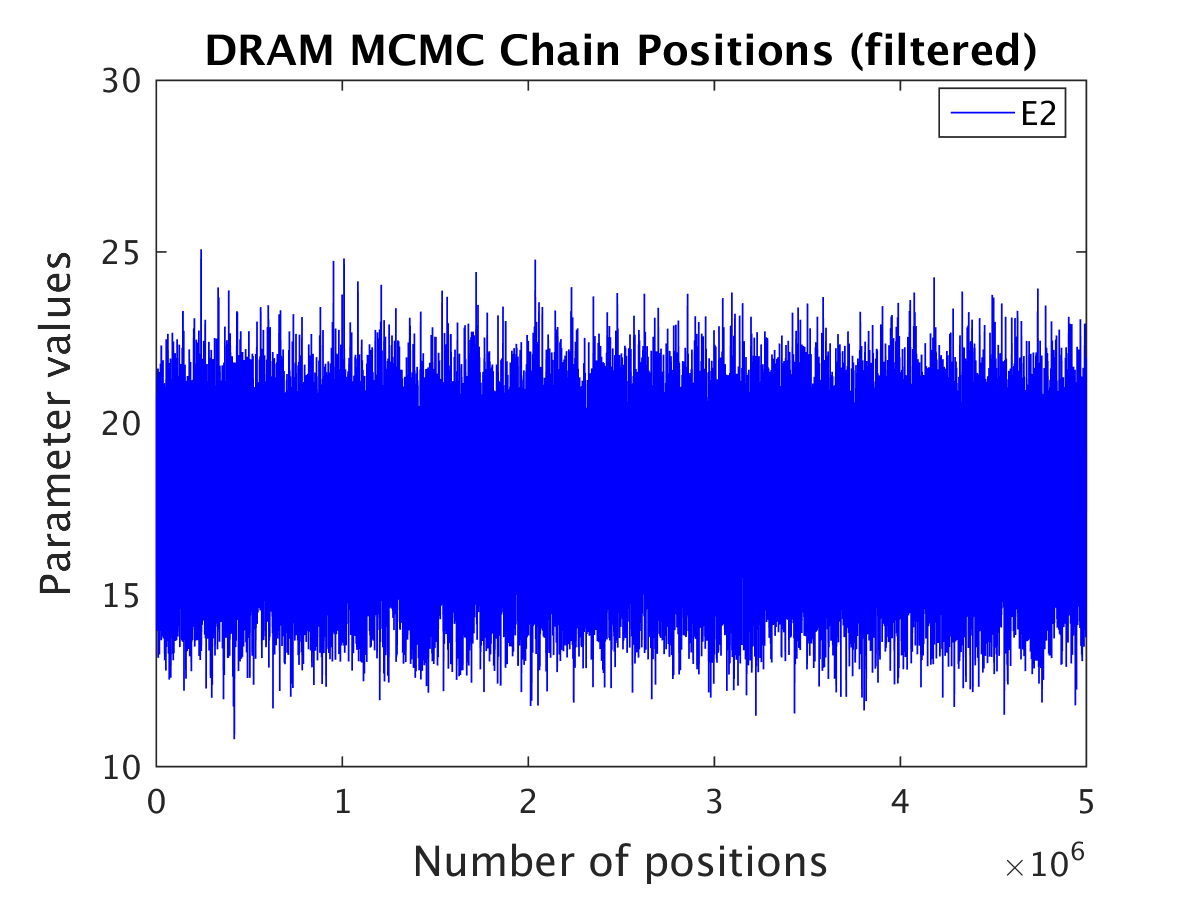
\includegraphics[scale=0.7]{multiple_data/20_kde/outputData_5e6/simple_ip_chain_pos_raw_1} 
    }
    \quad
    \subfloat[MCMC raw chain of samples of $E_2$\label{subfig-1:dummy}]{%
         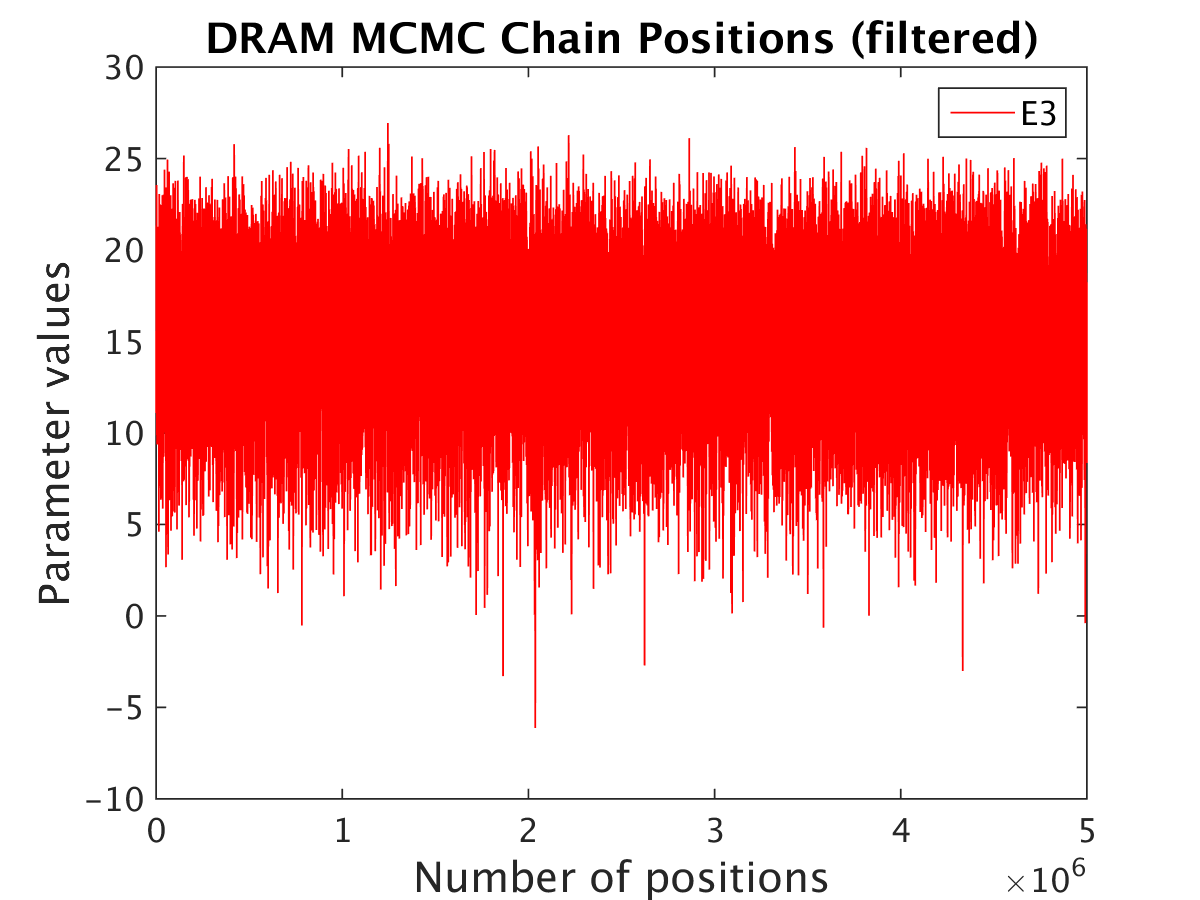
\includegraphics[scale=0.7]{multiple_data/20_kde/outputData_5e6/simple_ip_chain_pos_raw_2} 
        }
    \end{figure}
  \begin{figure}[H]
  \ContinuedFloat
  \centering
  \subfloat[Histogram for $E_2$ \label{subfig-1:dummy}]{%
       \includegraphics[scale=0.7]{multiple_data/20_kde/outputData_5e6/E2.pdf} 
      }
   \quad
    \subfloat[Histogram for $E_3$ \label{subfig-1:dummy}]{%
          \includegraphics[scale=0.7]{multiple_data/20_kde/outputData_5e6/E3.pdf} 
         }
\end{figure}
\begin{figure}[H]
  
   \subfloat[Cummulative Density Funtion \label{subfig-1:dummy}]{
        \includegraphics[scale=0.7]{multiple_data/20_kde/outputData_5e6/cdf} 
       }
     \quad
\subfloat[KDE \label{subfig-1:dummy}]{
        \includegraphics[scale=0.7]{multiple_data/20_kde/outputData_5e6/kde} 
            }  
  \caption{Results for sample size 5e6}
\end{figure}

\begin{figure}[H]
\centering
\subfloat[MCMC raw chain of samples of $E_2$\label{subfig-1:dummy}]{%
     \includegraphics[scale=0.7]{multiple_data/20_kde/outputData_1e7/simple_ip_chain_pos_raw_1} 
    }
    \quad
    \subfloat[MCMC raw chain of samples of $E_2$\label{subfig-1:dummy}]{%
         \includegraphics[scale=0.7]{multiple_data/20_kde/outputData_1e7/simple_ip_chain_pos_raw_2} 
        }
    \end{figure}
  \begin{figure}[H]
  \ContinuedFloat
  \centering
  \subfloat[Histogram for $E_2$ \label{subfig-1:dummy}]{%
       \includegraphics[scale=0.7]{multiple_data/20_kde/outputData_1e7/E2.pdf} 
      }
   \quad
    \subfloat[Histogram for $E_3$ \label{subfig-1:dummy}]{%
          \includegraphics[scale=0.7]{multiple_data/20_kde/outputData_1e7/E3.pdf} 
         }
\end{figure}
\begin{figure}[H]
  
   \subfloat[Cummulative Density Funtion \label{subfig-1:dummy}]{
        \includegraphics[scale=0.7]{multiple_data/20_kde/outputData_1e7/cdf} 
       }
     \quad
\subfloat[KDE \label{subfig-1:dummy}]{
        \includegraphics[scale=0.7]{multiple_data/20_kde/outputData_1e7/kde} 
            }  
  \caption{Results for sample size 1e7}
\end{figure}
\subsubsection{Sample size (Surrogate size) 30*30 }
In this section we calculated flamespeed values for 900 (30*30) different points in the domain and the remaining values are linear combination of these 900 points.  The results below are for sample size $1e5$, $5e5$ , $1e6$, $5e6$ and $1e7$. 

\begin{figure}[H]
\centering
\subfloat[MCMC raw chain of samples of $E_2$\label{subfig-1:dummy}]{%
     \includegraphics[scale=0.7]{multiple_data/30_kde/outputData_1e5/simple_ip_chain_pos_raw_1} 
    }
    \quad
    \subfloat[MCMC raw chain of samples of $E_2$\label{subfig-1:dummy}]{%
         \includegraphics[scale=0.7]{multiple_data/30_kde/outputData_1e5/simple_ip_chain_pos_raw_2} 
        }
    \end{figure}
  \begin{figure}[H]
  \ContinuedFloat
  \centering
  \subfloat[Histogram for $E_2$ \label{subfig-1:dummy}]{%
       \includegraphics[scale=0.7]{multiple_data/30_kde/outputData_1e5/E2.pdf} 
      }
   \quad
    \subfloat[Histogram for $E_3$ \label{subfig-1:dummy}]{%
          \includegraphics[scale=0.7]{multiple_data/30_kde/outputData_1e5/E3.pdf} 
         }
\end{figure}
\begin{figure}[H]
  
   \subfloat[Cummulative Density Funtion \label{subfig-1:dummy}]{
        \includegraphics[scale=0.7]{multiple_data/30_kde/outputData_1e5/cdf} 
       }
     \quad
\subfloat[KDE \label{subfig-1:dummy}]{
        \includegraphics[scale=0.7]{multiple_data/30_kde/outputData_1e5/kde} 
            }  
  \caption{Results for sample size 1e5}
\end{figure}

\begin{figure}[H]
\centering
\subfloat[MCMC raw chain of samples of $E_2$\label{subfig-1:dummy}]{%
     \includegraphics[scale=0.7]{multiple_data/30_kde/outputData_5e5/simple_ip_chain_pos_raw_1} 
    }
    \quad
    \subfloat[MCMC raw chain of samples of $E_2$\label{subfig-1:dummy}]{%
         \includegraphics[scale=0.7]{multiple_data/30_kde/outputData_5e5/simple_ip_chain_pos_raw_2} 
        }
    \end{figure}
  \begin{figure}[H]
  \ContinuedFloat
  \centering
  \subfloat[Histogram for $E_2$ \label{subfig-1:dummy}]{%
       \includegraphics[scale=0.7]{multiple_data/30_kde/outputData_5e5/E2.pdf} 
      }
   \quad
    \subfloat[Histogram for $E_3$ \label{subfig-1:dummy}]{%
          \includegraphics[scale=0.7]{multiple_data/30_kde/outputData_5e5/E3.pdf} 
         }
\end{figure}
\begin{figure}[H]
  
   \subfloat[Cummulative Density Funtion \label{subfig-1:dummy}]{
        \includegraphics[scale=0.7]{multiple_data/30_kde/outputData_5e5/cdf} 
       }
     \quad
\subfloat[KDE \label{subfig-1:dummy}]{
        \includegraphics[scale=0.7]{multiple_data/30_kde/outputData_5e5/kde} 
            }  
  \caption{Results for sample size 5e5}
\end{figure}


\begin{figure}[H]
\centering
\subfloat[MCMC raw chain of samples of $E_2$\label{subfig-1:dummy}]{%
     \includegraphics[scale=0.7]{multiple_data/30_kde/outputData_1e6/simple_ip_chain_pos_raw_1} 
    }
    \quad
    \subfloat[MCMC raw chain of samples of $E_2$\label{subfig-1:dummy}]{%
         \includegraphics[scale=0.7]{multiple_data/30_kde/outputData_1e6/simple_ip_chain_pos_raw_2} 
        }
    \end{figure}
  \begin{figure}[H]
  \ContinuedFloat
  \centering
  \subfloat[Histogram for $E_2$ \label{subfig-1:dummy}]{%
       \includegraphics[scale=0.7]{multiple_data/30_kde/outputData_1e6/E2.pdf} 
      }
   \quad
    \subfloat[Histogram for $E_3$ \label{subfig-1:dummy}]{%
          \includegraphics[scale=0.7]{multiple_data/30_kde/outputData_1e6/E3.pdf} 
         }
\end{figure}
\begin{figure}[H]
  
   \subfloat[Cummulative Density Funtion \label{subfig-1:dummy}]{
        \includegraphics[scale=0.7]{multiple_data/30_kde/outputData_1e6/cdf} 
       }
     \quad
\subfloat[KDE \label{subfig-1:dummy}]{
        \includegraphics[scale=0.7]{multiple_data/30_kde/outputData_1e6/kde} 
            }  
  \caption{Results for sample size 1e6}
\end{figure}


\begin{figure}[H]
\centering
\subfloat[MCMC raw chain of samples of $E_2$\label{subfig-1:dummy}]{%
     \includegraphics[scale=0.7]{multiple_data/30_kde/outputData_5e6/simple_ip_chain_pos_raw_1} 
    }
    \quad
    \subfloat[MCMC raw chain of samples of $E_2$\label{subfig-1:dummy}]{%
         \includegraphics[scale=0.7]{multiple_data/30_kde/outputData_5e6/simple_ip_chain_pos_raw_2} 
        }
    \end{figure}
  \begin{figure}[H]
  \ContinuedFloat
  \centering
  \subfloat[Histogram for $E_2$ \label{subfig-1:dummy}]{%
       \includegraphics[scale=0.7]{multiple_data/30_kde/outputData_5e6/E2.pdf} 
      }
   \quad
    \subfloat[Histogram for $E_3$ \label{subfig-1:dummy}]{%
          \includegraphics[scale=0.7]{multiple_data/30_kde/outputData_5e6/E3.pdf} 
         }
\end{figure}
\begin{figure}[H]
  
   \subfloat[Cummulative Density Funtion \label{subfig-1:dummy}]{
        \includegraphics[scale=0.7]{multiple_data/30_kde/outputData_5e6/cdf} 
       }
     \quad
\subfloat[KDE \label{subfig-1:dummy}]{
        \includegraphics[scale=0.7]{multiple_data/30_kde/outputData_5e6/kde} 
            }  
  \caption{Results for sample size 5e6}
\end{figure}

\begin{figure}[H]
\centering
\subfloat[MCMC raw chain of samples of $E_2$\label{subfig-1:dummy}]{%
     \includegraphics[scale=0.7]{multiple_data/30_kde/outputData_1e7/simple_ip_chain_pos_raw_1} 
    }
    \quad
    \subfloat[MCMC raw chain of samples of $E_2$\label{subfig-1:dummy}]{%
         \includegraphics[scale=0.7]{multiple_data/30_kde/outputData_1e7/simple_ip_chain_pos_raw_2} 
        }
    \end{figure}
  \begin{figure}[H]
  \ContinuedFloat
  \centering
  \subfloat[Histogram for $E_2$ \label{subfig-1:dummy}]{%
       \includegraphics[scale=0.7]{multiple_data/30_kde/outputData_1e7/E2.pdf} 
      }
   \quad
    \subfloat[Histogram for $E_3$ \label{subfig-1:dummy}]{%
          \includegraphics[scale=0.7]{multiple_data/30_kde/outputData_1e7/E3.pdf} 
         }
\end{figure}
\begin{figure}[H]
  
   \subfloat[Cummulative Density Funtion \label{subfig-1:dummy}]{
        \includegraphics[scale=0.7]{multiple_data/30_kde/outputData_1e7/cdf} 
       }
     \quad
\subfloat[KDE \label{subfig-1:dummy}]{
        \includegraphics[scale=0.7]{multiple_data/30_kde/outputData_1e7/kde} 
            }  
  \caption{Results for sample size 1e7}
\end{figure}
\subsubsection{Sample size (Surrogate size) 100*100 }
In this section we calculated flamespeed values for 10,000 (100*100) different points in the domain and the remaining values are linear combination of these 10,000 points.  The results below are for sample size $1e5$, $5e5$ , $1e6$, $5e6$ and $1e7$. 

\begin{figure}[H]
\centering
\subfloat[MCMC raw chain of samples of $E_2$\label{subfig-1:dummy}]{%
     \includegraphics[scale=0.7]{multiple_data/100_kde/outputData_1e5/simple_ip_chain_pos_raw_1} 
    }
    \quad
    \subfloat[MCMC raw chain of samples of $E_2$\label{subfig-1:dummy}]{%
         \includegraphics[scale=0.7]{multiple_data/100_kde/outputData_1e5/simple_ip_chain_pos_raw_2} 
        }
    \end{figure}
  \begin{figure}[H]
  \ContinuedFloat
  \centering
  \subfloat[Histogram for $E_2$ \label{subfig-1:dummy}]{%
       \includegraphics[scale=0.7]{multiple_data/100_kde/outputData_1e5/E2.pdf} 
      }
   \quad
    \subfloat[Histogram for $E_3$ \label{subfig-1:dummy}]{%
          \includegraphics[scale=0.7]{multiple_data/100_kde/outputData_1e5/E3.pdf} 
         }
\end{figure}
\begin{figure}[H]
  
   \subfloat[Cummulative Density Funtion \label{subfig-1:dummy}]{
        \includegraphics[scale=0.7]{multiple_data/100_kde/outputData_1e5/cdf} 
       }
     \quad
\subfloat[KDE \label{subfig-1:dummy}]{
        \includegraphics[scale=0.7]{multiple_data/100_kde/outputData_1e5/kde} 
            }  
  \caption{Results for sample size 1e5}
\end{figure}

\begin{figure}[H]
\centering
\subfloat[MCMC raw chain of samples of $E_2$\label{subfig-1:dummy}]{%
     \includegraphics[scale=0.7]{multiple_data/100_kde/outputData_5e5/simple_ip_chain_pos_raw_1} 
    }
    \quad
    \subfloat[MCMC raw chain of samples of $E_2$\label{subfig-1:dummy}]{%
         \includegraphics[scale=0.7]{multiple_data/100_kde/outputData_5e5/simple_ip_chain_pos_raw_2} 
        }
    \end{figure}
  \begin{figure}[H]
  \ContinuedFloat
  \centering
  \subfloat[Histogram for $E_2$ \label{subfig-1:dummy}]{%
       \includegraphics[scale=0.7]{multiple_data/100_kde/outputData_5e5/E2.pdf} 
      }
   \quad
    \subfloat[Histogram for $E_3$ \label{subfig-1:dummy}]{%
          \includegraphics[scale=0.7]{multiple_data/100_kde/outputData_5e5/E3.pdf} 
         }
\end{figure}
\begin{figure}[H]
  
   \subfloat[Cummulative Density Funtion \label{subfig-1:dummy}]{
        \includegraphics[scale=0.7]{multiple_data/100_kde/outputData_5e5/cdf} 
       }
     \quad
\subfloat[KDE \label{subfig-1:dummy}]{
        \includegraphics[scale=0.7]{multiple_data/100_kde/outputData_5e5/kde} 
            }  
  \caption{Results for sample size 5e5}
\end{figure}


\begin{figure}[H]
\centering
\subfloat[MCMC raw chain of samples of $E_2$\label{subfig-1:dummy}]{%
     \includegraphics[scale=0.7]{multiple_data/100_kde/outputData_1e6/simple_ip_chain_pos_raw_1} 
    }
    \quad
    \subfloat[MCMC raw chain of samples of $E_2$\label{subfig-1:dummy}]{%
         \includegraphics[scale=0.7]{multiple_data/100_kde/outputData_1e6/simple_ip_chain_pos_raw_2} 
        }
    \end{figure}
  \begin{figure}[H]
  \ContinuedFloat
  \centering
  \subfloat[Histogram for $E_2$ \label{subfig-1:dummy}]{%
       \includegraphics[scale=0.7]{multiple_data/100_kde/outputData_1e6/E2.pdf} 
      }
   \quad
    \subfloat[Histogram for $E_3$ \label{subfig-1:dummy}]{%
          \includegraphics[scale=0.7]{multiple_data/100_kde/outputData_1e6/E3.pdf} 
         }
\end{figure}
\begin{figure}[H]
  
   \subfloat[Cummulative Density Funtion \label{subfig-1:dummy}]{
        \includegraphics[scale=0.7]{multiple_data/100_kde/outputData_1e6/cdf} 
       }
     \quad
\subfloat[KDE \label{subfig-1:dummy}]{
        \includegraphics[scale=0.7]{multiple_data/100_kde/outputData_1e6/kde} 
            }  
  \caption{Results for sample size 1e6}
\end{figure}


\begin{figure}[H]
\centering
\subfloat[MCMC raw chain of samples of $E_2$\label{subfig-1:dummy}]{%
     \includegraphics[scale=0.7]{multiple_data/100_kde/outputData_5e6/simple_ip_chain_pos_raw_1} 
    }
    \quad
    \subfloat[MCMC raw chain of samples of $E_2$\label{subfig-1:dummy}]{%
         \includegraphics[scale=0.7]{multiple_data/100_kde/outputData_5e6/simple_ip_chain_pos_raw_2} 
        }
    \end{figure}
  \begin{figure}[H]
  \ContinuedFloat
  \centering
  \subfloat[Histogram for $E_2$ \label{subfig-1:dummy}]{%
       \includegraphics[scale=0.7]{multiple_data/100_kde/outputData_5e6/E2.pdf} 
      }
   \quad
    \subfloat[Histogram for $E_3$ \label{subfig-1:dummy}]{%
          \includegraphics[scale=0.7]{multiple_data/100_kde/outputData_5e6/E3.pdf} 
         }
\end{figure}
\begin{figure}[H]
  
   \subfloat[Cummulative Density Funtion \label{subfig-1:dummy}]{
        \includegraphics[scale=0.7]{multiple_data/100_kde/outputData_5e6/cdf} 
       }
     \quad
\subfloat[KDE \label{subfig-1:dummy}]{
        \includegraphics[scale=0.7]{multiple_data/100_kde/outputData_5e6/kde} 
            }  
  \caption{Results for sample size 5e6}
\end{figure}

\begin{figure}[H]
\centering
\subfloat[MCMC raw chain of samples of $E_2$\label{subfig-1:dummy}]{%
     \includegraphics[scale=0.7]{multiple_data/100_kde/outputData_1e7/simple_ip_chain_pos_raw_1} 
    }
    \quad
    \subfloat[MCMC raw chain of samples of $E_2$\label{subfig-1:dummy}]{%
         \includegraphics[scale=0.7]{multiple_data/100_kde/outputData_1e7/simple_ip_chain_pos_raw_2} 
        }
    \end{figure}
  \begin{figure}[H]
  \ContinuedFloat
  \centering
  \subfloat[Histogram for $E_2$ \label{subfig-1:dummy}]{%
       \includegraphics[scale=0.7]{multiple_data/100_kde/outputData_1e7/E2.pdf} 
      }
   \quad
    \subfloat[Histogram for $E_3$ \label{subfig-1:dummy}]{%
          \includegraphics[scale=0.7]{multiple_data/100_kde/outputData_1e7/E3.pdf} 
         }
\end{figure}
\begin{figure}[H]
  
   \subfloat[Cummulative Density Funtion \label{subfig-1:dummy}]{
        \includegraphics[scale=0.7]{multiple_data/100_kde/outputData_1e7/cdf} 
       }
     \quad
\subfloat[KDE \label{subfig-1:dummy}]{
        \includegraphics[scale=0.7]{multiple_data/100_kde/outputData_1e7/kde} 
            }  
  \caption{Results for sample size 1e7}
\end{figure}


\subsection{Convergence Study }

\noindent In this section, we see the convergence of the probability distribution as we increase the raw chain sample size. The plot is done for surrogate size of 100. In this analysis, raw chain size of $1e5$, $5e5$ , $1e6$, $5e6$ and $1e7$ is taken. 

\begin{figure}[H]
\centering
\subfloat[ Convergence  \label{subfig-1:dummy}]{
\includegraphics[scale=0.7]{multiple_data/100_kde/convergence_study/conv} 
  }
    \caption{Convergence for surrogate size 100}
\end{figure}


\subsection{flamespeed Data fit}

\noindent It is necessary to ensure that the samples of the parameters which we are drawing are fitting the flamespeed values of the experimental. In this section, we calculate the flamespeed for all the parameters drawn using the surrogate generated before. We have taken $1e7$ sample size and calculated flamespeed for different concentrations of ozone. 

\begin{figure}[H]
\centering
\subfloat[ Flame speed for 20 \% ozone   \label{subfig-1:dummy}]{
\includegraphics[scale=0.7]{multiple_data/flamespeed_calculation/flame_20.pdf} 
  }
  \quad
  \subfloat[ Flame speed for 28 \% ozone   \label{subfig-1:dummy}]{
  \includegraphics[scale=0.7]{multiple_data/flamespeed_calculation/flame_28.pdf} 
    }
\end{figure}


 \begin{figure}[H]
  \ContinuedFloat
  \centering
   \subfloat[ Flame speed for 40 \% ozone \label{subfig-1:dummy}]{
        \includegraphics[scale=0.7]{multiple_data/flamespeed_calculation/flame_40.pdf} 
       }
     \quad
\subfloat[Flame speed for 46 \% ozone \label{subfig-1:dummy}]{
        \includegraphics[scale=0.7]{multiple_data/flamespeed_calculation/flame_46.pdf} 
            }  
\end{figure}


 \begin{figure}[H]
  \ContinuedFloat
  \centering
   \subfloat[ Flame speed for 53 \% ozone \label{subfig-1:dummy}]{
        \includegraphics[scale=0.7]{multiple_data/flamespeed_calculation/flame_53.pdf} 
       }
     \quad
\subfloat[Flame speed for 75 \% ozone \label{subfig-1:dummy}]{
        \includegraphics[scale=0.7]{multiple_data/flamespeed_calculation/flame_75.pdf} 
            }  
\end{figure}


 \begin{figure}[H]
  \ContinuedFloat
  \centering
   \subfloat[ Flame speed for 100 \% ozone \label{subfig-1:dummy}]{
        \includegraphics[scale=0.7]{multiple_data/flamespeed_calculation/flame_100.pdf} 
       }
  \caption{Flamespeed Data fit}
\end{figure}